\documentclass[11pt]{article}

\usepackage[utf8]{inputenc}
\usepackage[T1]{fontenc}
\usepackage{amsmath,amssymb,amsthm}
\usepackage{booktabs}
\usepackage{graphicx}
\usepackage{hyperref}
\usepackage[capitalize,noabbrev]{cleveref}
\usepackage[margin=1in]{geometry}
\usepackage{pgfplots}
\pgfplotsset{compat=1.18}
\usepackage{natbib}
\usepackage{xcolor}

\hypersetup{
    colorlinks=true,
    linkcolor=blue,
    citecolor=blue,
    urlcolor=blue
}

\title{LayerNorm as Implicit Gain Control in Looped Transformers}
\author{Matthias M.\ M.\ Buehlmaier\\
\textit{Faculty of Business and Economics, The University of Hong Kong}\\
\textit{Pokfulam Road, Hong Kong}\\
\texttt{buehl@hku.hk}}
\date{July 12, 2026}

\begin{document}

\maketitle

\begin{abstract}
In pre-LayerNorm looped transformers, LayerNorm inside the recurrent block acts as an implicit gain controller: by coupling the block's local Lipschitz constant inversely to the activation scale, it renders the recurrence Jacobian non-normal---asymptotically contractive at every verified fixed point even where its operator norm exceeds 1---so the true stability budget is the spectral margin, not an operator-norm bound. That margin depletes as the carry $\rho \to 1$, and a minority of initializations never converge to a fixed point at all, so the diagonal carry constraint $\rho(\bar{A}) < 1$ is necessary but not sufficient for convergence of the full recurrence. Training experiments across six tasks, including a controlled ablation, reveal that the linear carry is not the depth-memory mechanism: gradient descent routes memory through the block's more expressive nonlinear recurrence and leaves the stability-constrained carry at rest---the carry's role is stabilization, not memory. We characterize the boundary of this claim: on tasks with axis-aligned per-channel structure, gradient descent does recruit the carry. All results are derived analytically and verified in a from-scratch, CPU-scale implementation; verification at larger scale is needed.
\end{abstract}


\section{Introduction}

Looped transformers---architectures that reuse a single block of transformer weights across multiple depth iterations---decouple reasoning depth from parameter count, offering substantial inference-time savings. A model with $k$ unique layers iterated $T$ times achieves the effective depth of a $kT$-layer network while storing only the $k$ shared layers' weights. At fixed quality this translates into large parameter savings: \citet{parcae2026} report matching a Transformer's quality with roughly half the parameters. This makes the architecture attractive for deployment at scale, where inference costs dominate and parameter efficiency translates directly to serving economics.

However, the training cost remains comparable to conventional transformers of equivalent effective depth. Each iteration of the shared block contributes to the forward pass and must be backpropagated through, so the FLOP budget scales with effective depth regardless of parameter sharing. The savings are in memory (fewer unique weights) and inference (smaller model to serve), not in the training compute required to learn those weights.

This asymmetry has a practical consequence: looped transformers will be deployed primarily by organizations that can afford frontier-scale training runs---and stability failures during such runs are disproportionately costly. A single training divergence at 70B parameters wastes weeks of compute time and hundreds of thousands of dollars. Understanding the stability properties of the recurrent-depth architecture at small scale, before committing to expensive training runs, is therefore not merely pedagogical but economically necessary.

This paper contributes three previously uncharacterized stability properties of looped transformers with pre-LayerNorm blocks:

\textbf{First}, LayerNorm inside the recurrent block acts as an implicit gain controller, coupling the block's local Lipschitz constant inversely to the activation scale: the increment's Lipschitz constant tracks $1-\rho$ (the affine dependence $\rho + \tfrac{C}{F}(1-\rho)$ is derived, with the constant of proportionality $C/F \approx 2.5$ measured near-constant across carries). This coupling does \emph{not} pin an operator-norm bound near 1---that bound descends from $\approx$2 to 1 as $\rho \to 1$, and the measured operator norm itself exceeds 1 at low carry---but it renders the recurrence Jacobian \emph{non-normal}: across 10 random-weight seeds, every instance that converges to a fixed point has operator norm above 1 there (measured at $\rho = 0.3$ and $0.9$; all five carries for a representative instance) while its spectral radius stays below 1. The true stability budget is the spectral margin $1-\rho_{\text{spec}}(J_G)$, collapsing monotonically from $0.159$ at $\rho = 0.3$ to $0.012$ at $\rho = 0.95$; moreover, a minority of untrained instances never converge to a fixed point at all (1/10 at low carry, 2/10 from $\rho = 0.7$; the trajectory remains on a bounded, non-settling orbit)---so the diagonal carry constraint bounds the linear part but does not by itself certify convergence of the full recurrence. We measure both $\rho_{\text{spec}}$ and the operator norm by power iteration on Jacobian--vector products (validated matrix-free against dense), a finite-difference Lipschitz probe under-estimating the operator norm $\approx$2.6-fold along the block's dense direction (\cref{sec:lipschitz,sec:self-stabilization}). We derive the relationship analytically, verify it empirically across carry values from 0.3 to 0.95, and identify the activation-implosion failure mode where small activation norms cause the Lipschitz constant to spike (\cref{sec:implosion}).

\textbf{Second}, under per-channel carry, the system's stability margin is governed by the single slowest channel, revealing a memory-stability tradeoff on the depth axis that is mathematically identical to the tradeoff governing diagonal state-space models (S4, Mamba) on the sequence axis (\cref{sec:per-channel}).

\textbf{Third}---and most consequentially---in all cross-channel tasks tested, the linear carry is not the depth-memory mechanism. The block's nonlinear recurrence through the hidden state is more expressive and incurs no observed stability cost, so gradient descent routes memory through it and leaves the carry at rest---or actively lowers it, because smaller $\bar{A}$ gives faster convergence of the fixed-point iteration without sacrificing any memory the block can't already provide. However, on a task with axis-aligned per-channel structure, gradient descent does recruit the carry---characterizing the boundary of the claim. Since natural-language tasks are overwhelmingly cross-channel, Parcae's spectral-radius constraint is low-cost in practice. The constraint remains necessary: removing it allows gradient descent to drive $\rho(\bar{A}) > 1$ at higher learning rates, reproducing Parcae's core instability finding at toy scale. The carry's role is stabilization, not memory (\cref{sec:training}).

All results are derived analytically and verified empirically at small scale ($d=8$--$32$, 2--4 heads, sequence lengths 1--32, CPU only) using a from-scratch implementation in Clojure with hand-derived, finite-difference-verified backpropagation. The analytical claims are dimension-independent; the training experiments are confirmed by controlled ablation. The theoretical basis for the central finding---that the block's nonlinear recurrence is more expressive than a diagonal scaling on the region where states live---suggests it generalizes, but verification at larger scale and on richer tasks is needed.

\paragraph{Relationship to Parcae.} The default implementation studies a Parcae-inspired gated recurrent-depth transformer, not a faithful reproduction. Deviations: no explicit $\bar{B} \cdot e$ linear injection (input enters only through the nonlinear block), no prelude normalization, $\Delta = 1$ fixed (not learned), fixed loop depth (no stochastic depth sampling). These deviations are provably irrelevant to the claims. The omitted terms ($\bar{B} \cdot e$, prelude $\text{LN}(e)$) are functions of the input $e$, which is constant across the $T$ loop iterations and therefore has zero Jacobian with respect to $h_t$. Learnable $\Delta$ is a reparameterization of the diagonal carry ($\rho = \max \bar{A}$ still governs stability). We confirm empirically: a faithful implementation including $\bar{B} \cdot e$, learnable $\Delta$, and prelude normalization reproduces the central windowed-copy result identically.


\section{Related Work}
\label{sec:related}

\textbf{Parcae}~\citep{parcae2026} identifies two stability mechanisms---a spectral-norm constraint on the diagonal state-transition matrix (which we call the carry) and prelude normalization. Our finding adds a third---implicit gain control from LayerNorm---and shows it is dominant at the operating point. The training experiments suggest why Parcae's constraint works well: gradient descent does not use the linear carry for memory.

\textbf{S4/Mamba}~\citep{s4,mamba}: The constrained discretization Parcae imports from S4---which builds on HiPPO's optimal-projection memory~\citep{hippo} and was later reduced to a diagonal, and then scalar, state matrix~\citep{s4d,mamba2}---guarantees $\rho < 1$. Our result concerns the nonlinear term S4 lacks. The interaction is specific to the looped setting: in standard (non-looped) transformers, LayerNorm's $1/\|x\|$ property exists but has no recurrence to stabilize. The per-channel analysis (\cref{sec:per-channel}) shows the memory-stability tradeoff governing S4/Mamba's diagonal state matrix transfers intact to the depth-recurrence axis.

\textbf{Parcae's test-time scaling law}~\citep[§5.3]{parcae2026} fits $\mathcal{L}(T) = \mathcal{L}_\infty + Ze^{-zT}$ and notes a ``nice connection'' to their dynamical systems framework. The contraction mapping analysis in \cref{sec:self-stabilization} makes this connection explicit: the fixed-point iteration converges at an effective local rate $r_\text{eff}$---asymptotically the \emph{spectral radius} of the full recurrence Jacobian (the carry \emph{plus} the block's Jacobian $\partial f/\partial h$), not the carry $\rho$ alone; we measure this spectral radius directly (\cref{tab:spectral,tab:seed-robustness}) and find it exceeds the carry $\rho$ at every operating point---so convergence is slower than the carry alone predicts---and rises toward $1$ as $\rho \to 1$, with a minority of initializations ($1$--$2$ of $10$ across the carries tested) never converging to a fixed point at all (the probed $\text{Lip}(G)$ of the probe record (\cref{app:probe-record}) does \emph{not} bound the rate---being a finite-difference lower bound it falls below $\rho_{\text{spec}}$; only the true operator norm upper-bounds it; see the norm/spectral-radius hierarchy in \cref{subsec:directional}). Each additional loop iteration then refines the hidden state by a factor $\approx r_\text{eff}$, giving diminishing returns at a predictable exponential rate. The spiral geometry we observe---shrinking steps in rotating directions---is the mechanism behind their saturating exponential. This also explains why the decay rate in Parcae's unified law scales as $z/\mu_\text{rec}$: models trained at higher mean recurrence learn dynamics with larger effective $r_\text{eff}$ (slower convergence, longer time constants), producing shallower decay curves at test time.

\textbf{Looped transformers for reasoning}~\citep{saunshi2025,geiping2025,kohli2026}: A parallel line of work studies recurrent-depth architectures as a substrate for latent reasoning. \citet{saunshi2025} show a $k$-layer transformer looped $L$ times nearly matches a $kL$-layer network on reasoning tasks and can simulate chain-of-thought in latent space; \citet{geiping2025} scale test-time recurrence to a 3.5B-parameter model; and \citet{kohli2026} demonstrate systematic generalization and depth extrapolation under implicit reasoning. These works motivate looping to greater depth at test time; our stability analysis characterizes the dynamical regime that keeps such looping well-behaved.

\textbf{Adaptive Computation Time}~\citep{graves2016} solves when to stop looping. The activation-implosion finding has implications: if an ACT halting criterion uses activation-based signals, the small-$\|h\|$ regime could produce pathological decisions precisely when dynamics are least reliable.


\section{Setup and Notation}
\label{sec:setup}

Consider the Parcae recurrence for a looped transformer:
\begin{equation}
h_{t+1} = \bar{A} \odot h_t + f(h_t, e)
\label{eq:recurrence}
\end{equation}
where:
\begin{itemize}
    \item $h_t \in \mathbb{R}^{n \times d}$ is the hidden state at loop iteration $t$ (sequence length $\times$ embedding dim)
    \item $\bar{A} = \exp(\Delta t \cdot (-\exp(\log\_A))) \in (0,1)^d$ is the constrained diagonal carry (per Parcae). In the general case, $\log\_A \in \mathbb{R}^d$ is a learnable vector giving per-channel carry rates; the scalar case ($\log\_A \in \mathbb{R}$, broadcast to all channels) is a special case.
    \item $e$ is the encoded input from the Prelude, re-injected each iteration
    \item $f$ is the transformer block \emph{increment}---the block's output minus its input, $f(h_t,e) = \text{Block}(h_t + e) - (h_t + e)$, comprising pre-LN multi-head self-attention and pre-LN MLP. The block's internal residual (identity) path is carried by the $\bar{A} \odot h_t$ term, so $f$ contains no identity in $h_t$; its Jacobian is $\partial f / \partial h_t = \partial u / \partial h_t$ where $u$ is the sublayer increment (see \cref{app:coupling})
\end{itemize}

We write $\rho = \|\bar{A}\|_\infty$ for the spectral radius (= max diagonal entry, since $\bar{A}$ is diagonal with positive entries).

\textbf{Norms and indexing.} Unless flagged otherwise, $\|\cdot\|$ on states denotes the Frobenius norm over positions and channels; LayerNorm statistics $\mu, \sigma$ are per token. In per-channel expressions such as \cref{eq:fixed-point}, $(h^*_i)^2$ abbreviates the squared norm of channel $i$ aggregated over positions.

Parcae's stability argument: $\rho < 1$ by construction, which bounds the linear component. The nonlinear block $f$ is treated as a perturbation that prelude normalization and training regularization must keep in check.

We show that pre-LayerNorm does more than ``keep $f$ in check''---it actively couples the system to the stability boundary.


\section{The Lipschitz Structure of LayerNorm}
\label{sec:lipschitz}

LayerNorm maps $x \mapsto \gamma \odot \frac{x - \mu}{\sigma} + \beta$, where $\mu, \sigma$ are per-token statistics.

\textbf{Key property:} For a pre-LN block, the effective Lipschitz constant of the block with respect to its input scales inversely with the per-token spread: $\text{Lip}(f) \propto 1/\sigma(h) = 1/\sqrt{\text{Var}(h) + \varepsilon}$, where $\text{Var}(h)$ is the centered per-token variance and $\varepsilon$ caps the singularity as $\sigma \to 0$. Since $\sigma \le \text{RMS}(h)$ with equality when the per-token mean is small (and exactly $1/\text{RMS}(h)$ for RMSNorm, which omits centering), we report against $\|H\|$ (RMS) below as a proxy; the two coincide except for tokens concentrated near the all-ones direction. The inverse coupling is not specific to LayerNorm's algebraic form: it follows from degree-0 homogeneity (scale invariance) of the normalizer alone (\cref{app:coupling}). A second caveat on the proxy: LayerNorm acts per token, so the operator-norm-relevant scale is the \emph{smallest} per-token spread; reporting against a single global $\|H\|$ presumes token spreads scale together (\cref{sec:implosion} returns to this). Concretely, we observe empirically:

\begin{table}[ht]
\centering
\begin{tabular}{@{}cccc@{}}
\toprule
$\|H\|$ (RMS) & Lip(block) & Lip(increment) & $\|H\| \times$ Lip(increment) \\
\midrule
$\sim$2 & $\sim$17 & $\sim$17 & $\sim$36 \\
$\sim$11 & $\sim$3.1 & $\sim$2.9 & $\sim$31 \\
$\sim$44 & $\sim$1.2 & $\sim$0.65 & $\sim$28 \\
$\sim$218 & $\sim$1.0 & $\sim$0.12 & $\sim$27 \\
\bottomrule
\end{tabular}
\caption{Lipschitz constant of a pre-LN transformer block scales inversely with activation norm. LayerNorm divides by standard deviation, which scales with $\|x\|$. The last column exhibits the coupling directly: the product $\|H\| \times \text{Lip(increment)}$ is the constant $C$ of \cref{app:coupling}, near-constant across two orders of magnitude in $\|H\|$; its $\approx$25\% drift reflects the direction dependence of $C$ and the RMS-vs-spread proxy gap. These Lip values are finite-difference probes; the true operator norms (power iteration) are larger by a factor comparable to that in \cref{tab:cf}, which rescales $C$ but preserves both its near-constancy and the $\text{Lip} \propto 1/\|H\|$ scaling this table demonstrates.}
\label{tab:lipschitz-scaling}
\end{table}

This is not surprising in isolation---LayerNorm divides by the standard deviation, which scales with $\|x\|$. What is surprising is how precisely this interacts with the carry.

\subsection{Verification: Banach Contraction Threshold}

Before applying the Lipschitz framework to the full transformer block, we verified it on a minimal system: the Parcae recurrence with $f(h, e) = \tanh(\text{gain} \cdot Wh + e)$ for a random $8 \times 8$ matrix $W$, at $\rho = 0.368$ (plus a constant $\bar{B} \odot e$ injection, which has zero Jacobian in $h$ and does not enter the contraction condition). The Banach fixed-point theorem~\citep{granas2003} guarantees convergence when $\rho + \text{gain} \cdot \|W\|_\sigma < 1$, where $\|W\|_\sigma$ is the spectral norm. For the specific sampled $W$ used here the measured $\|W\|_\sigma \approx 5.39$ (power iteration; close to the $\approx 2\sqrt{8} \approx 5.66$ asymptotic for $8 \times 8$ i.i.d.\ $\mathcal{N}(0,1)$ entries), giving a guaranteed-convergence region gain $< (1 - 0.368)/5.39 \approx 0.117$.

Empirically, the loop converges to a stable fixed point at gain $\leq 0.25$ and wanders without settling at gain $\geq 0.30$: the observed threshold sits roughly $2\times$ above the Banach sufficient condition. The gap has a concrete source: the bound charges $\tanh$ its global slope of $1$, whereas at the fixed point the pre-activations $\text{gain} \cdot Wh^* + e$ are not small, so the local slope---and with it the effective Lipschitz constant---is strictly smaller. The Banach condition is thus confirmed as a valid but conservative sufficient condition for the gated recurrence with a nonlinear block---the same sufficient-not-necessary structure that the operator-norm analysis of \cref{sec:self-stabilization} exhibits at full block scale.


\section{The Self-Stabilization Result}
\label{sec:self-stabilization}

\subsection{Fixed-Point Scale Law}

At the fixed point $h^*$ of the gated recurrence, the balance condition $f(h^*, e) = (I - \text{diag}(\bar{A}))\,h^*$ holds componentwise, i.e.\ $f_i = (1 - \bar{A}_i)\,h^*_i$. Taking norms:
\begin{equation}
\|f(h^*, e)\|^2 = \sum_i (1 - \bar{A}_i)^2 (h^*_i)^2,
\qquad\text{so}\qquad
(1 - \rho)\|h^*\| \;\le\; \|f(h^*, e)\| \;\le\; (1 - \min_i \bar{A}_i)\|h^*\|.
\label{eq:fixed-point}
\end{equation}
For a \emph{scalar} carry $\bar{A} = \rho I$ the bounds collapse to the exact balance equation $(1-\rho)\|h^*\| = \|f(h^*, e)\|$; in the per-channel case the equality holds only when $h^*$ concentrates in the slowest ($\max_i \bar{A}_i$) channel. The carry's contraction thus matches the increment's injection up to this channel spread.

It is cleaner to state the per-channel case as an \emph{exact} identity. Writing $D = \text{diag}(\bar{A})$ and the state-weighted contraction factor
\begin{equation}
q_D(h^*) := \frac{\|(I - D)\,h^*\|}{\|h^*\|}
= \left(\frac{\sum_i (1 - \bar{A}_i)^2 (h^*_i)^2}{\sum_i (h^*_i)^2}\right)^{1/2},
\qquad 1 - \rho \;\le\; q_D(h^*) \;\le\; 1 - \min_i \bar{A}_i,
\label{eq:qd}
\end{equation}
the balance condition gives $\|f(h^*, e)\| = q_D(h^*)\,\|h^*\|$ exactly, so the fixed-point scale obeys $\|h^*\| = F/q_D(h^*)$ with $F := \|f(h^*, e)\|$. The slowest channel dominates $q_D$ (and thus governs the fixed-point scale) only when $h^*$ carries substantial mass in it; $q_D = 1 - \rho$ exactly in the scalar case. The worst-case bound $\|h^*\| \le F/(1-\rho)$ follows since $\|f\|$ is approximately constant (LayerNorm normalizes internal activations), i.e.\ $\|h^*\| = O\!\big(1/(1-\rho)\big)$. This matches the scalar toy model's prediction, verified to 3 significant figures. (The worst-case $\rho = \max_i \bar{A}_i$ governs the operator-norm Banach bound; the fixed-point \emph{scale} is governed by $q_D(h^*)$; and actual local stability by $\|D + J_f(h^*)\|$, developed next.)

\paragraph{Existence and an unconditional scale bound.} The identities above presuppose a fixed point; existence does not require contraction. Every path through the increment passes through a normalizer, whose output is bounded independently of its input ($\|\text{LN}(x)\| \le \|\gamma\|_\infty \sqrt{d} + \|\beta\|$ per token), so the increment is uniformly bounded: $\|f(h,e)\| \le B$ with $B$ determined by the weights and dimensions, not by $h$ (\cref{app:existence}). Hence $G$ maps the closed ball $\|h\| \le B/(1-\rho)$ into itself, and Brouwer's fixed-point theorem~\citep{granas2003} guarantees a fixed point $h^*$ with $\|h^*\| \le B/(1-\rho)$---the $O(1/(1-\rho))$ scale law as an a priori bound, independent of the empirical near-constancy of $\|f\|$ at $h^*$. Uniqueness and local stability are separate questions, governed by $J_G(h^*)$ below.

The approach to the fixed point exhibits the spiral geometry reported by Parcae: step sizes $\|h_{t+1} - h_t\|$ decay overall (2.44 $\to$ 0.06 over 16 iterations), with a small transient rebound around $t \approx 8$, while successive update directions become increasingly orthogonal (cosine similarity with the first update sweeps from 1.0 through 0.0 to $-0.63$ and back). Shrinking steps in rotating directions describe a spiral---a signature of contraction in a space where the Jacobian has complex-like eigenstructure (\cref{fig:spiral}). This geometry is a property of the contractive dynamics themselves, not of learned weights: it appears identically with random initialization. Two distinct inferences must be kept apart here. The spiral evidences complex (rotational) eigenstructure of the local Jacobian but is silent on \emph{non-normality}: a normal scaled rotation $rR(\theta)$ spirals while its operator norm equals its spectral radius. The step-size rebound, by contrast, is suggestive of non-normal transient amplification---under an exactly linear contraction with a normal Jacobian, step norms decay monotonically---though at $t \approx 8$ the trajectory may sit outside the linearization's reach, so we flag rather than claim it (\cref{subsec:directional}).

\begin{figure}[ht]
\centering
\begin{minipage}{0.44\textwidth}
\centering
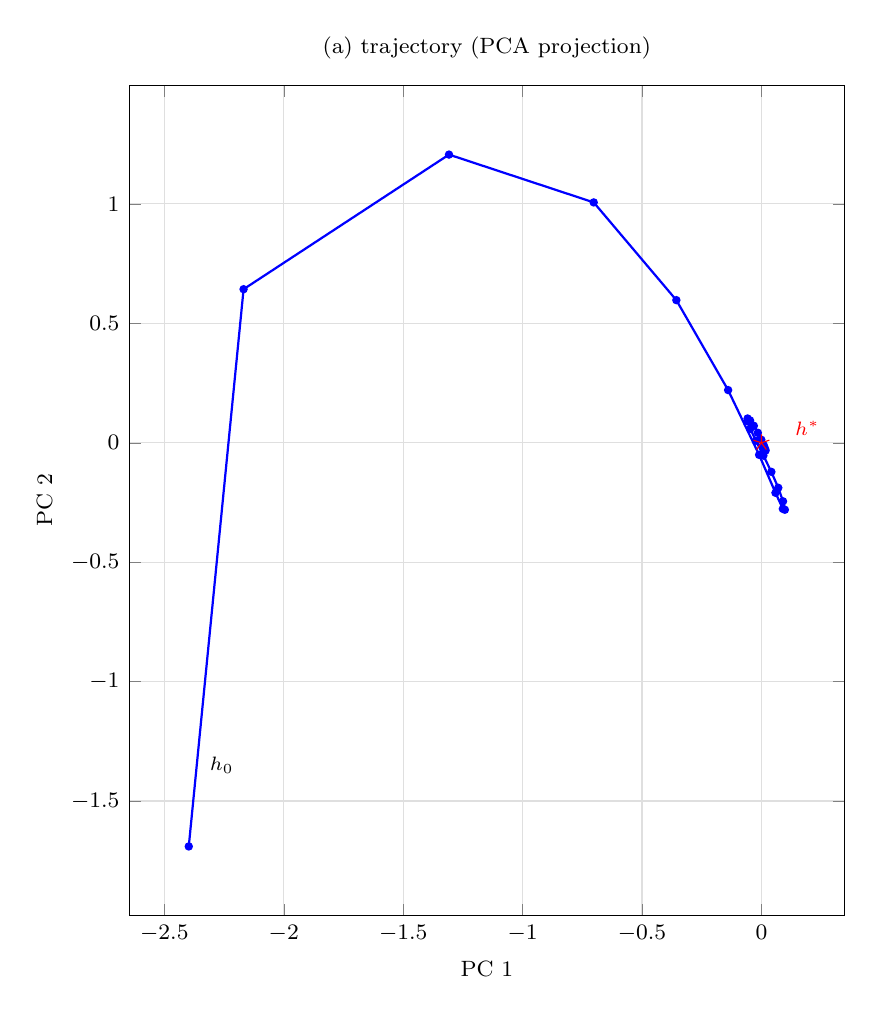
\begin{tikzpicture}
\begin{axis}[
    width=\textwidth,
    height=\textwidth,
    axis equal image,
    title={(a) trajectory (PCA projection)},
    xlabel={PC 1}, ylabel={PC 2},
    grid=major, grid style={gray!25},
    tick label style={font=\footnotesize},
    label style={font=\footnotesize},
    title style={font=\footnotesize},
]
% 2D PCA projection of the d=8 nonlinear loop (gain 0.25), centered on the fixed point.
\addplot[blue, thick, mark=*, mark size=1.1pt, mark options={fill=blue}] coordinates {
    (-2.3978,-1.6901) (-2.1683,0.6430) (-1.3083,1.2066) (-0.7023,1.0064)
    (-0.3563,0.5972) (-0.1396,0.2207) (-0.0098,-0.0505) (0.0587,-0.2093)
    (0.0896,-0.2765) (0.0979,-0.2804) (0.0903,-0.2451) (0.0704,-0.1884)
    (0.0414,-0.1217) (0.0081,-0.0536) (-0.0233,0.0087) (-0.0468,0.0586)
    (-0.0586,0.0905) (-0.0580,0.1017) (-0.0477,0.0935) (-0.0319,0.0711)
    (-0.0152,0.0418) (-0.0006,0.0127) (0.0099,-0.0109) (0.0157,-0.0262)
    (0.0172,-0.0327) (0.0152,-0.0315) (0.0107,-0.0246) (0.0050,-0.0144)
};
\addplot[red, mark=star, mark size=3pt, only marks] coordinates {(0,0)};
\node[anchor=west, font=\scriptsize] at (axis cs:-2.35,-1.35) {$h_0$};
\node[anchor=west, font=\scriptsize, red] at (axis cs:0.10,0.06) {$h^*$};
\end{axis}
\end{tikzpicture}
\end{minipage}\hfill
\begin{minipage}{0.54\textwidth}
\centering
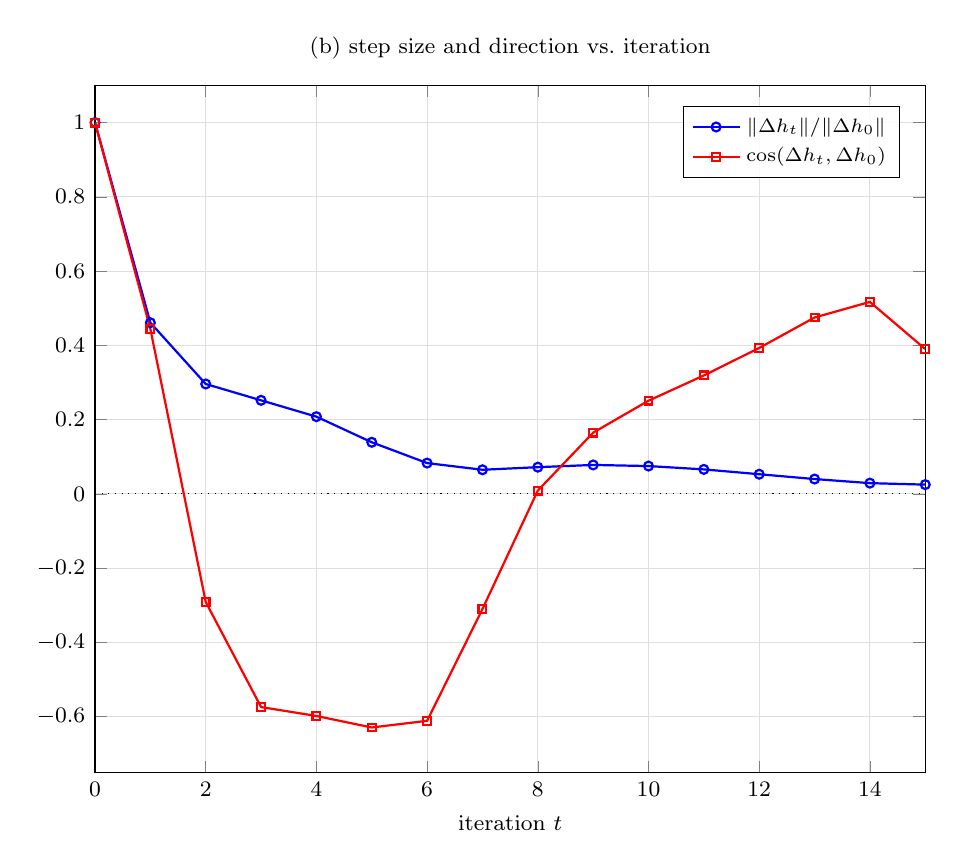
\begin{tikzpicture}
\begin{axis}[
    width=\textwidth,
    height=0.85\textwidth,
    title={(b) step size and direction vs.\ iteration},
    xlabel={iteration $t$},
    xmin=0, xmax=15,
    ymin=-0.75, ymax=1.1,
    legend pos=north east,
    legend style={font=\scriptsize, fill opacity=0.85, text opacity=1},
    grid=major, grid style={gray!25},
    tick label style={font=\footnotesize},
    label style={font=\footnotesize},
    title style={font=\footnotesize},
]
\addplot[black, dotted, sharp plot, mark=none, forget plot] coordinates {(0,0) (15,0)};
% step size normalized by the first step (2.437): shrinking
\addplot[blue, thick, mark=o, mark size=1.6pt] coordinates {
    (0,1.000) (1,0.461) (2,0.296) (3,0.252) (4,0.208) (5,0.139) (6,0.083)
    (7,0.065) (8,0.072) (9,0.078) (10,0.075) (11,0.066) (12,0.053)
    (13,0.040) (14,0.029) (15,0.025)
};
\addlegendentry{$\|\Delta h_t\| / \|\Delta h_0\|$}
% cosine of each update vs the first: rotating (sweeps to $-0.63$ and back)
\addplot[red, thick, mark=square, mark size=1.4pt] coordinates {
    (0,1.000) (1,0.444) (2,-0.291) (3,-0.574) (4,-0.598) (5,-0.629) (6,-0.611)
    (7,-0.310) (8,0.009) (9,0.165) (10,0.251) (11,0.319) (12,0.393)
    (13,0.475) (14,0.517) (15,0.390)
};
\addlegendentry{$\cos(\Delta h_t, \Delta h_0)$}
\end{axis}
\end{tikzpicture}
\end{minipage}
\caption{Spiral geometry of the contractive loop ($d=8$ toy, $f(h,e)=\tanh(Wh+e)$ with random $W$, gain 0.25, $\rho=0.368$). \textbf{(a)} The trajectory projected onto its top two principal components spirals into the fixed point $h^*$. \textbf{(b)} Step size (blue) decays overall---note the small transient rebound around $t \approx 8$, suggestive of non-normal amplification (\cref{subsec:directional})---while the update direction (red) rotates: its cosine against the first update sweeps from 1.0 through 0 to $-0.63$ and back. Shrinking steps in rotating directions is the signature of contraction with complex-like Jacobian eigenstructure.}
\label{fig:spiral}
\end{figure}

\subsection{Marginal Stability: Operator Norm vs.\ Spectral Radius}

Write the local inverse-norm coupling as $\text{Lip}(f)|_{h} = C/\|h\|$ for a constant $C$ (the operator-norm scale of $\partial f/\partial h$ times $\|h\|$; see \cref{app:coupling}). We combine this with the \emph{exact} scale identity $\|h^*\| = F/q_D(h^*)$ (\cref{eq:qd}), $F := \|f(h^*,e)\|$---not the worst-case bound $\|h^*\| \le F/(1-\rho)$---to obtain
\begin{equation}
\text{Lip}(f)\big|_{h=h^*} = \frac{C}{\|h^*\|} = \frac{C}{F}\,q_D(h^*)
\;\xrightarrow{\text{scalar carry}}\;
\frac{C}{F}\,(1 - \rho).
\label{eq:lip-coupling}
\end{equation}
The choice of identity over bound is deliberate: the worst-case scale $\|h^*\| \le F/(1-\rho)$ yields only a \emph{lower} bound $\text{Lip}(f)|_{h^*} \gtrsim \tfrac{C}{F}(1-\rho)$, which cannot by itself support an upper bound on $\text{Lip}(G)$. Since $1-\rho \le q_D(h^*) \le 1-\min_i\bar{A}_i$ (\cref{eq:qd}), the reduction to $1-\rho$ is exact in the scalar case and holds otherwise only when $h^*$ concentrates its mass in the slowest channel. The total Lipschitz bound on the gated map $G(h) = \bar{A} \odot h + f(h, e)$ is then, in the scalar-carry case,
\begin{equation}
\text{Lip}(G) \leq \rho + \text{Lip}(f) \approx \rho + \frac{C}{F}(1 - \rho)
\qquad\text{(per-channel: replace $1-\rho$ by $q_D(h^*)$)}.
\label{eq:marginal}
\end{equation}
The derivation fixes the \emph{affine} form $\rho + \tfrac{C}{F}(1-\rho) = \tfrac{C}{F} + \big(1 - \tfrac{C}{F}\big)\rho$, interpolating between $C/F$ at $\rho = 0$ and exactly $1$ at $\rho = 1$. Two consequences follow \emph{regardless} of the value of $C/F$: the bound approaches $1$ as $\rho \to 1$ (riding the boundary at high carry is structural, not calibrated), and it is flat across all $\rho$ if and only if $C/F = 1$. The value of the constant is an empirical question. Measuring the increment's true local Lipschitz constant $\text{Lip}(f)|_{h^*} = \|J_f(h^*)\|_2$ by power iteration (\cref{tab:cf}) gives $C/F = \text{Lip}(f)/(1-\rho) \approx 2.5$, near-constant across $\rho \in [0.3, 0.95]$ (range $2.33$--$2.78$). The functional relationship is thus confirmed---$C/F$ is a genuine constant and $\text{Lip}(f)$ tracks $(1-\rho)$, the LayerNorm inverse-norm coupling verified directly---and with $C/F \approx 2.5$ the Banach bound is $\rho + 2.5\,(1-\rho)$, descending from $\approx 2$ at low carry to $1$ as $\rho \to 1$. It is \emph{not} flat near $1$ and exceeds $1$ everywhere except in the $\rho \to 1$ limit: the operator-norm sum does not certify contraction at any carry short of that limit. (An axis-aware finite-difference probe would instead imply $C/F \approx 1$: it under-samples the block's dense top singular direction and under-estimates $\|J_f\|_2$ by $\approx 2.6\times$; the probe record is retained in \cref{app:probe-record}.) Strictly, neither $F = \|f(h^*,e)\|$ nor $C$ is a true constant: $F$ varies with the fixed-point direction, the input injection $e$, the attention pattern, and $\rho$; $C$ varies with the normalized direction through the softmax and activation derivatives; LayerNorm makes $F$ plausibly $O(1)$ but does not pin it. What survives is the derived \emph{scalar functional form} plus an empirically calibrated constant $C/F \approx 2.5$. Self-stabilization is therefore real but operates one level down: the inverse-norm coupling keeps the \emph{spectral radius} of the full Jacobian below and near $1$ (\cref{subsec:directional}), not the operator-norm sum. For per-channel carry the relation holds with $q_D(h^*)$ (\cref{eq:qd}) in place of $1-\rho$; since $q_D$ can sit far above $1-\rho$---a single channel at $\bar{A}_i = 0.99$ with state mass spread across channels gives $q_D \approx 0.5$ and a bound well above $1$---the per-channel Banach bound certifies even less, and observed stability rests on the spectral radius together with the directional slack $\delta$ of the next subsection (cf.\ \cref{tab:per-channel}).

\begin{table}[ht]
\centering
\begin{tabular}{@{}ccccc@{}}
\toprule
$\rho$ & true $\text{Lip}(f) = \|J_f\|_2$ & probed $\text{Lip}(f)$ & $F = \|f(h^*,e)\|$ & $C/F = \text{Lip}(f)/(1-\rho)$ \\
\midrule
0.30 & 1.628 & 0.608 & 22.84 & 2.33 \\
0.50 & 1.233 & 0.463 & 22.99 & 2.47 \\
0.70 & 0.833 & 0.303 & 23.22 & 2.78 \\
0.90 & 0.239 & 0.093 & 26.66 & 2.39 \\
0.95 & 0.119 & 0.046 & 27.22 & 2.38 \\
\bottomrule
\end{tabular}
\caption{The self-stabilization constant $C/F$, measured. The increment's true local Lipschitz constant $\|J_f(h^*)\|_2$ (top singular value by power iteration on the materialized Jacobian) tracks $(1-\rho)$---confirming the LayerNorm inverse-norm coupling---with a near-constant ratio $C/F = \text{Lip}(f)/(1-\rho) \approx 2.5$, \emph{not} $\approx 1$. The fixed-point balance $F = (1-\rho)\|h^*\|$ holds to the displayed precision (balance ratio $1.000$ at every carry, at a residual-verified fixed point), so $C/F = \|J_f\|_2\,\|h^*\|/F = \|J_f\|_2/(1-\rho)$. The finite-difference probe (third column) under-estimates $\|J_f\|_2$ by $\approx 2.6\times$, which is why a probe-based estimate implies $C/F \approx 1$ (probe record: \cref{app:probe-record}). We confirmed the true $\|J_f\|_2$ independently by perturbing the increment map along its recovered top singular direction. $d=32$, seq $16$, random weights.}
\label{tab:cf}
\end{table}

\subsection{Actual Contraction: The Directional Margin}
\label{subsec:directional}

An axis-aware finite-difference probe of $\text{Lip}(G)$ sits below 1 at every carry (probe record: \cref{app:probe-record})---but such probes are lower bounds, and the true operator norm can exceed 1 (\cref{tab:spectral}); the Banach sub-additive bound is not tight along the directions the probe samples. The carry $\bar{A}$ is diagonal; the increment's Jacobian is dense (attention + MLP). Their top singular directions do not align, so the triangle-inequality worst-case (where both amplify the same direction simultaneously) is not realized---though, as \cref{tab:spectral} shows, the residual $\|J_G\|_2$ still exceeds 1 at low carry, and it is $\rho_{\text{spec}} < 1$, not the operator norm, that certifies contraction there.

This can be made a measurable identity rather than an intuition. Write $J_G = D + J_f$ with $J_f := \partial f/\partial h\,(h^*, e)$ and $D = \text{diag}(\bar{A})$ (so $\|D\|_2 = \rho$). Define the contraction margin $m := 1 - \|J_G\|_2$ and the triangle-inequality slack from directional misalignment
\begin{equation}
\delta := \|D\|_2 + \|J_f\|_2 - \|D + J_f\|_2 \;\ge\; 0.
\end{equation}
Then $m = 1 - \rho - \|J_f\|_2 + \delta$: the Banach budget depleted by $\rho + \|J_f\|_2$ is recovered in part by the alignment slack $\delta$, and operator-norm contraction ($m > 0$) requires the recovered slack to exceed the nominal excess $\rho + \|J_f\|_2 - 1$. Measured, this excess is \emph{not} covered at low carry: with true operator norms (\cref{tab:cf,tab:spectral}), $\rho + \|J_f\|_2 \approx 1.93$ and $\delta \approx 0.19$ at $\rho = 0.3$, so $m = 1 - \|J_G\|_2 \approx -0.74 < 0$---the operator norm does not certify contraction there. The ``directional margin'' of the probe record (\cref{app:probe-record}) reports $1 - \text{probed Lip}(G)$, positive only because the finite-difference probe under-estimates $\|J_G\|_2$; it is not the true operator-norm margin $m$. The directional slack $\delta$ is real but modest and does not by itself pull the operator norm below $1$; what certifies contraction is the additional \emph{inner} gap down to the spectral radius, measured next.

The full picture is a two-slack hierarchy,
\begin{equation}
\rho_{\text{spec}}(J_G) \;\le\; \|J_G\|_2 \;\le\; \|D\|_2 + \|J_f\|_2 = \rho + \|J_f\|_2,
\label{eq:hierarchy}
\end{equation}
whose outer gap is the directional (triangle-inequality) slack $\delta$ measured above, and whose inner gap is governed by the non-normality of $J_G$ and is not measured here. The probed $\text{Lip}(G)$ approximates the middle quantity \emph{from below}---finite-difference probes lower-bound the operator norm---while the asymptotic per-iteration convergence rate of the fixed-point iteration (the $r_\text{eff}$ of Parcae's test-time scaling law, \cref{sec:related}) is the spectral radius $\rho_{\text{spec}}(J_G(h^*))$, upper-bounded by the \emph{true} operator norm $\|J_G\|_2$. We measure all three by power iteration on Jacobian--vector products---central-difference JVPs of the forward map $G$ (matrix-free), with $\rho_{\text{spec}}$ read off as the geometric mean of the per-step growth $\|J_G^k v\|^{1/k}$ (Gelfand's formula, robust to the complex eigenstructure the spiral implies) and $\|J_G\|_2$ as the top singular value of the densely materialized Jacobian; the matrix-free and dense $\rho_{\text{spec}}$ estimates agree to $\le 0.004$ (\cref{tab:spectral}). Three findings result (\cref{tab:spectral} reports one representative instance, seed 7; \cref{tab:seed-robustness} the seed distribution). First, for this instance $\rho_{\text{spec}}(J_G) < 1$ at every carry, so the loop is asymptotically contractive---the guarantee behind the observed convergence and the saturating-exponential scaling law (across seeds this holds for \emph{every} instance that converges to a fixed point; a minority never converge at all, \cref{tab:seed-robustness}). Second, $J_G$ is markedly \emph{non-normal}: the true $\|J_G\|_2$ exceeds $1$ at low and moderate carry ($1.74$ at $\rho=0.3$, $1.30$ at $\rho=0.7$) while $\rho_{\text{spec}}$ sits at $0.90$--$0.96$, so a perturbation is transiently amplified before it contracts---the quantitative datum behind the step-size rebound of \cref{fig:spiral}b. The non-normality gap $\|J_G\|_2-\rho_{\text{spec}}$ is largest at low carry ($0.81$ at $\rho=0.3$) and closes as $\rho\to1$ ($0.03$ at $\rho=0.95$), where the near-normal diagonal carry dominates $J_G$. Third, the finite-difference probe under-estimates $\|J_G\|_2$ so severely (e.g.\ $0.85$ vs.\ a true $1.74$ at $\rho=0.3$, which we confirmed by directly perturbing $G$ along the recovered top singular direction) that the probe falls \emph{below} $\rho_{\text{spec}}$ at every operating point. The probe record's operator-norm ``directional margin'' (\cref{app:probe-record}) is therefore an artifact of that probe slack, not a contraction certificate: the true operator norm affords no margin at low carry. Asymptotic stability is instead certified by the spectral margin $1-\rho_{\text{spec}}$, positive at every $\rho$ for this instance (widest, $\approx 0.10$, near $\rho=0.5$) but narrowing to $0.013$ at $\rho=0.95$; averaged over the seeds that converge, the margin is widest at low carry ($0.159$ at $\rho=0.3$) and collapses monotonically to $0.012$ as $\rho \to 1$ (\cref{tab:seed-robustness}), the single-instance non-monotonicity sitting within the seed spread. Power iteration on JVPs thus cleanly separates the asymptotic convergence rate from the worst-case transient amplification, which are numerically far apart in this regime.

\textbf{Methodological note:} Naive random-direction perturbation underestimates $\text{Lip}(G)$ for diagonal-carry maps in high dimensions. Random vectors have negligible weight on any single coordinate axis, missing axis-aligned worst cases. All values below use axis-aware (robust) Lipschitz estimation: probing both random directions and each channel axis independently, taking the maximum. Homogeneity adds a structural caveat: the normalizer's Jacobian annihilates its own input direction ($J_{\text{LN}}(x)\,x = 0$ at $\varepsilon = 0$; \cref{app:coupling}), so the component of a probe parallel to the block input $h + e$ contributes nothing through the normalizer path---a second, independent way naive probing underestimates. Even axis-aware probing, however, misses a \emph{third} and here dominant case: the top singular direction of the dense increment Jacobian $J_f$ is a coupled, non-axis-aligned direction that neither random nor channel-axis probes sample, so the probe still under-estimates $\|J_f\|_2$ (hence $\|J_G\|_2$) by $\approx 2.6\times$ (\cref{tab:cf,tab:spectral}). Crucially, this miss is specific to the dense direction: the axis-aligned carry direction \emph{is} captured by the channel-axis probes, so the per-channel worst-axis margins of \cref{sec:per-channel} are unaffected by it. The full finite-difference probe record is retained for methodological comparison in \cref{app:probe-record}.

\begin{figure}[ht]
\centering
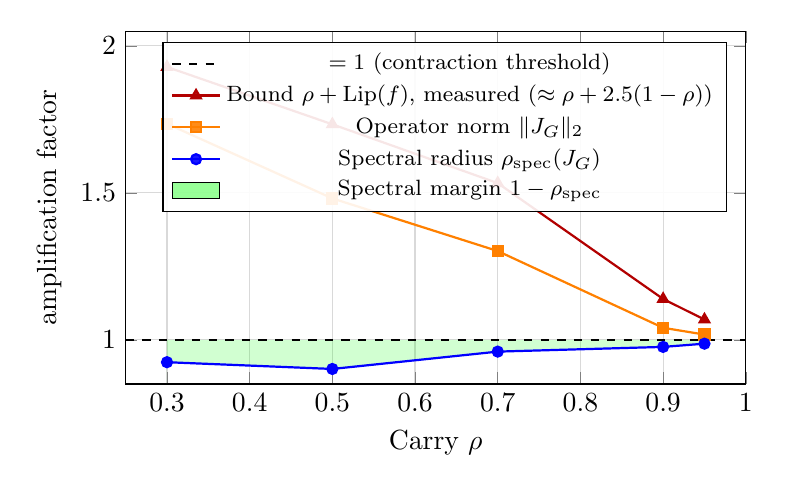
\begin{tikzpicture}
\begin{axis}[
    width=0.78\textwidth,
    height=0.5\textwidth,
    xlabel={Carry $\rho$},
    ylabel={amplification factor},
    xmin=0.25, xmax=1.0,
    ymin=0.85, ymax=2.05,
    legend pos=north east,
    legend style={font=\footnotesize, fill opacity=0.9, text opacity=1},
    grid=major,
    grid style={gray!30},
]
% shaded spectral margin: between rho_spec and 1 (the true stability budget)
\addplot[green!50!black, fill=green, fill opacity=0.18, draw=none, forget plot] coordinates {
    (0.3, 0.924) (0.5, 0.901) (0.7, 0.960) (0.9, 0.976) (0.95, 0.987)
    (0.95, 1.0) (0.9, 1.0) (0.7, 1.0) (0.5, 1.0) (0.3, 1.0)
} \closedcycle;
\addplot[black, dashed, thick, sharp plot, mark=none] coordinates {(0.25, 1.0) (1.0, 1.0)};
\addlegendentry{$=1$ (contraction threshold)}
\addplot[red!70!black, thick, mark=triangle*, mark size=2pt] coordinates {
    (0.3, 1.928) (0.5, 1.733) (0.7, 1.533) (0.9, 1.139) (0.95, 1.069)
};
\addlegendentry{Bound $\rho + \mathrm{Lip}(f)$, measured ($\approx \rho + 2.5(1-\rho)$)}
\addplot[orange, thick, mark=square*, mark size=1.8pt] coordinates {
    (0.3, 1.735) (0.5, 1.481) (0.7, 1.302) (0.9, 1.041) (0.95, 1.018)
};
\addlegendentry{Operator norm $\|J_G\|_2$}
\addplot[blue, thick, mark=*, mark size=1.8pt] coordinates {
    (0.3, 0.924) (0.5, 0.901) (0.7, 0.960) (0.9, 0.976) (0.95, 0.987)
};
\addlegendentry{Spectral radius $\rho_{\text{spec}}(J_G)$}
\addlegendimage{area legend, draw=none, fill=green, fill opacity=0.4}
\addlegendentry{Spectral margin $1-\rho_{\text{spec}}$}
\end{axis}
\end{tikzpicture}
\caption{The two-slack stability picture---representative instance (seed 7; $d=32$, seq $16$; validated by direct perturbation). The Banach bound $\rho + \text{Lip}(f) = \rho + 2.5(1-\rho)$ (top) and the true operator norm $\|J_G\|_2$ (middle) both exceed 1 at low and moderate carry and descend toward 1 only as $\rho \to 1$; the spectral radius $\rho_{\text{spec}}(J_G)$ (bottom) alone stays below 1 for this instance. The shaded spectral margin $1 - \rho_{\text{spec}}$ is the stability budget; for this seed it peaks near $\rho \approx 0.5$, but averaged over the seeds that converge it is widest at low carry and collapses monotonically as $\rho \to 1$ ($0.159 \to 0.012$; \cref{tab:seed-robustness}). (A finite-difference probe would instead suggest a flat operator-norm margin sitting just under 1---an artifact of the probe under-estimating $\|J_G\|_2$ by $\approx 2.6\times$; probe record in \cref{app:probe-record}.)}
\label{fig:marginal-stability}
\end{figure}

\begin{table}[ht]
\centering
\begin{tabular}{@{}cccccc@{}}
\toprule
$\rho$ & $\rho_{\text{spec}}(J_G)$ & $\|J_G\|_2$ & probed Lip($G$) & $\|J_G\|_2 - \rho_{\text{spec}}$ & spectral margin $1-\rho_{\text{spec}}$ \\
\midrule
0.30 & 0.924 & 1.735 & 0.850 & 0.811 & 0.076 \\
0.50 & 0.901 & 1.481 & 0.826 & 0.580 & 0.099 \\
0.70 & 0.960 & 1.302 & 0.852 & 0.342 & 0.040 \\
0.90 & 0.976 & 1.041 & 0.937 & 0.065 & 0.024 \\
0.95 & 0.987 & 1.018 & 0.968 & 0.031 & 0.013 \\
\bottomrule
\end{tabular}
\caption{Spectral radius vs.\ operator norm of the recurrence Jacobian $J_G(h^*)$, by power iteration on Jacobian--vector products (matrix-free central-difference JVPs; $d=32$, seq $16$, random weights, same block as \cref{tab:cf}). $\rho_{\text{spec}} < 1$ everywhere---the loop is asymptotically contractive---while the \emph{true} $\|J_G\|_2 > 1$ at low and moderate carry: $J_G$ is non-normal, and the gap (the inner gap of the hierarchy, \cref{eq:hierarchy}) closes as $\rho \to 1$. The finite-difference probed Lip($G$) (\cref{app:probe-record}) under-estimates $\|J_G\|_2$ badly---it even falls below $\rho_{\text{spec}}$---so the load-bearing stability quantity is the spectral margin $1-\rho_{\text{spec}}$, not an operator-norm margin. The matrix-free $\rho_{\text{spec}}$ agrees with a dense-Jacobian Gelfand cross-check to $\le 0.004$. All rows are measured at a residual-verified fixed point (relative residual $< 10^{-9}$).}
\label{tab:spectral}
\end{table}

\begin{table}[ht]
\centering
\begin{tabular}{@{}ccccc@{}}
\toprule
$\rho$ & $\rho_{\text{spec}}(J_G)$ (mean $\pm$ std) & spectral margin $1-\rho_{\text{spec}}$ & with $\rho_{\text{spec}} > 1$ & non-convergent \\
\midrule
0.30 & $0.841 \pm 0.062$ & 0.159 & 0/9 & 1/10 \\
0.50 & $0.896 \pm 0.046$ & 0.104 & 0/9 & 1/10 \\
0.70 & $0.947 \pm 0.033$ & 0.053 & 0/8 & 2/10 \\
0.90 & $0.974 \pm 0.009$ & 0.026 & 0/8 & 2/10 \\
0.95 & $0.988 \pm 0.004$ & 0.012 & 0/8 & 2/10 \\
\bottomrule
\end{tabular}
\caption{Seed robustness of the spectral radius (10 random-weight initializations; matrix-free power iteration at residual-verified fixed points, relative residual $< 10^{-9}$; cross-checked against the dense Jacobian at $\rho = 0.3, 0.9$, means agreeing to $\le 0.004$). Statistics are over the seeds that converge to a fixed point (the denominators in column four); the final column counts the seeds that never do---their trajectories remain on bounded, non-settling orbits (relative residual $10^{-4}$--$10^{-1}$ after $2 \times 10^4$ iterations, neither decaying nor diverging), so there is no settled state at which to evaluate the Jacobian. Every instance that converges is contractive at its fixed point ($\rho_{\text{spec}} < 1$ in all rows), and the spectral margin collapses monotonically from $0.159$ at low carry to $0.012$ as $\rho \to 1$. \emph{Non-convergence, not marginal expansion, is the observed failure mode}: one initialization in ten fails to converge already at low carry, two in ten from $\rho = 0.7$. By contrast the operator norm $\|J_G\|_2 > 1$ in every converged instance at both $\rho = 0.3$ (mean $1.88$, $9/9$) and $\rho = 0.9$ (mean $1.07$, $8/8$): non-normality is universal.}
\label{tab:seed-robustness}
\end{table}

\paragraph{The diagonal constraint is necessary but not sufficient.} That a subset of initializations never converges to a fixed point, while the Parcae carry itself satisfies $\rho(\bar{A}) < 1$ by construction, isolates a gap the constraint does not close: bounding the \emph{linear} part of the recurrence does not certify convergence of the \emph{full} map $G(h) = \bar{A} \odot h + f(h,e)$, whose dense nonlinear term can sustain a bounded, non-settling orbit. The failure mode is starker than marginal expansion at a fixed point: a fixed point \emph{exists} for these initializations (Brouwer guarantees existence unconditionally, \cref{app:existence}), but it is not attracting from the initial condition used---the iteration circulates instead of settling, and its relative residual plateaus at $10^{-4}$--$10^{-1}$ rather than decaying. Every initialization that does converge is contractive at its fixed point ($\rho_{\text{spec}} < 1$ without exception, \cref{tab:seed-robustness}), so the dichotomy across seeds is convergent-and-contractive versus non-convergent, not a gradual crossing of $\rho_{\text{spec}} = 1$. The failures are present already at low carry ($1/10$ at $\rho = 0.3$) and become more frequent at high carry ($2/10$ from $\rho = 0.7$), where the shrinking spectral margin of the convergent instances compounds the risk. It sharpens the economic motivation of the introduction: convergence failures are not merely possible in principle but present in $1$--$2$ of $10$ random initializations here, and the right training-time diagnostic is the loop's own convergence---the residual $\|G(h)-h\|$ across iterations, together with $\rho_{\text{spec}}(J_G)$ at the settled state---not $\rho(\bar{A}) < 1$ alone. Whether gradient descent steers toward or away from these configurations is a training-dynamics question (\cref{sec:training}); we note only that the learned carry there stays low (\cref{tab:tinyshakes,tab:windowed-copy}), i.e.\ in the regime where the spectral margin of convergent instances is widest---consistent with, though not proof of, the optimizer keeping models off the thin-margin high-carry edge.

\subsection{Per-Channel Carry and the Memory-Stability Tradeoff}
\label{sec:per-channel}

When $\log\_A$ is a learnable vector rather than a scalar, each embedding dimension $i$ has its own carry $\bar{A}_i \in (0,1)$ and therefore its own effective memory horizon $\tau_i = 1/(1-\bar{A}_i)$ (the geometric-sum horizon $\sum_t \bar{A}_i^t$; the exact discrete e-folding time is $-1/\ln \bar{A}_i$, which agrees with $\tau_i$ as $\bar{A}_i \to 1$ but differs for small carry---e.g.\ $0.83$ vs.\ $1.4$ at $\bar{A}_i = 0.3$). This creates a bank of memory horizons: fast channels ($\bar{A}_i \approx 0.3$, $\tau \approx 1.4$) track the latest refinement; slow channels ($\bar{A}_i \approx 0.99$, $\tau \approx 100$) integrate long-range state.

The worst-axis (operator-norm) margin, however, is governed by $\max_i(\bar{A}_i)$:

\begin{table}[ht]
\centering
\begin{tabular}{@{}cccc@{}}
\toprule
Carry profile & Mean $\rho$ & Max $\rho$ & Worst-axis margin \\
\midrule
Uniform 0.5 (scalar) & 0.50 & 0.50 & 0.17 \\
31 channels at 0.5, 1 at 0.99 & 0.515 & 0.99 & 0.011 \\
Ramp 0.5 $\to$ 0.99 across 32 channels & 0.745 & 0.99 & 0.010 \\
Uniform 0.99 (scalar) & 0.99 & 0.99 & 0.006 \\
\bottomrule
\end{tabular}
\caption{A single slow channel pins the \emph{worst-axis (operator-norm)} margin to $\approx$0.01 regardless of other channels---no stability discount from sparsity in the Banach worst case. This diagnoses the linear path along its worst axis; the full map's margin there may be lower still or partially rescued by directional misalignment (\cref{eq:marginal} ff.), so it is a worst-case diagnostic, not a full stability theorem.}
\label{tab:per-channel}
\end{table}

This reveals a fundamental duality: \textbf{the channel with the longest memory horizon is the channel with the tightest stability margin.} The optimizer, in learning $\log\_A$, implicitly navigates this tradeoff per dimension---pushing a channel toward $\bar{A}_i = 1$ to capture long-range dependencies silently erodes that channel's stability margin toward zero. \Cref{eq:marginal} sharpens the danger: with mixed profiles the Banach bound $\rho + \tfrac{C}{F}q_D(h^*)$ generally exceeds $1$ (the slow channel contributes $\rho \approx 1$ while $q_D$ reflects the full state distribution), so the slow channel operates where the bound certifies nothing and stability there is carried by directional misalignment alone.

This recapitulates, on the depth-recurrence axis, the core design tension in diagonal SSMs (S4, S4D, Mamba): the eigenvalue closest to the unit circle provides the most memory and the least stability margin. The mathematical structure is identical, with only the axis of recurrence (depth vs.\ sequence position) differing.

\textbf{Training diagnostic:} Monitor $\max_i(\bar{A}_i)$, not the mean. If the optimizer drives any channel toward 1, the certified contraction margin approaches zero along that axis.


\section{The Activation-Implosion Failure Mode}
\label{sec:implosion}

The $1/\|h\|$ scaling of $\text{Lip}(f)$ creates an asymmetric risk profile:

\begin{itemize}
    \item \textbf{Large activations $\to$ safe.} $\text{Lip}(f)$ drops, margin grows, loop is firmly contractive.
    \item \textbf{Small activations $\to$ dangerous.} $\text{Lip}(f)$ spikes ($\sim$17 at $\|h\|\approx 2$ vs.\ $\sim$0.1 at $\|h\|\approx 218$) and contraction is no longer certified. Strictly, a failed sufficient condition does not by itself imply expansion---but the directional slack $\delta$ measured at healthy operating points is $\approx 0.19$ (\cref{subsec:directional}), which cannot absorb a Lipschitz excess of order $16$, so the loop becomes locally expansive.
\end{itemize}

This predicts a failure mode distinct from residual explosion: \textbf{activation implosion followed by divergence.} If training dynamics drive recurrent-block activations toward zero, the Lipschitz constant spikes, contraction fails, and gradients explode---from below, not above.

Practically, monitoring $\|h\|$ in the recurrent block during training is a direct early-warning signal: a sustained drop in activation scale precedes instability, with a lead time predictable from the $1/(1-\rho)$ time constant. Because LayerNorm acts per token, the binding quantity is the \emph{smallest per-token spread} $\min_{\text{token}} s(h)$: a single imploded token spikes the block's local Lipschitz constant even while the global norm looks healthy. The global $\|h\|$ is a convenient proxy; the per-token minimum is the sharper early-warning signal.

Parcae independently identifies the complementary failure mode: at 1.3B scale, growing prelude output norms destabilize the first loop iteration from above~\citep[Fig.~21--22]{parcae2026}. Together, these bracket the stable operating regime: activations must remain large enough for LayerNorm's gain control (our finding) and small enough that input injection does not overwhelm the carry (Parcae's finding).

We now turn to whether training dynamics preserve or break this self-stabilizing regime.


\section{Training Dynamics}
\label{sec:training}

The results in \cref{sec:lipschitz,sec:self-stabilization} are established at initialization. The central question is whether gradient descent preserves the self-stabilizing regime or breaks it.

The section follows one arc. We first remove the carry constraint to establish the instability it prevents (\cref{subsec:unconstrained}), then test whether gradient descent recruits the carry across tasks of increasing memory demand and specificity---a language-modeling null result (\cref{subsec:tinyshakes}), a falsified full-attention copy prediction (\cref{subsec:full-attn}), and the decisive windowed-copy experiment (\cref{subsec:windowed}). The arc culminates in an ablation that isolates the actual depth-memory mechanism (\cref{subsec:ablation}) and a constructed boundary case that maps exactly when the carry \emph{is} recruited (\cref{subsec:boundary}).

\subsection{Unconstrained Carry: Reproducing the Instability}
\label{subsec:unconstrained}

To establish the baseline, we compare the Parcae-constrained carry ($\bar{A} = \exp(-\exp(\log\_A)) \in (0,1)$) against an unconstrained free scalar carry across learning rates on Tiny Shakespeare ($d=24$, $T=8$, 120 steps).

\begin{table}[ht]
\centering
\begin{tabular}{@{}lcccc@{}}
\toprule
 & lr=$10^{-3}$ & lr=$10^{-2}$ & lr=$3 \times 10^{-2}$ & lr=$10^{-1}$ \\
\midrule
Parcae $\rho(\bar{A})$ & 0.512 & 0.606 & 0.790 & 0.777 \\
Free $\rho(\bar{A})$ & 0.534 & 0.755 & 1.197 & 1.841 \\
Free $\|h_T\|$ & 4.0 & 31 & 325 & 9,570 \\
\bottomrule
\end{tabular}
\caption{Unconstrained carry learns $\rho > 1$ at higher learning rates, with residual state explosion. Reproduces Parcae's Table 2 / Fig.\ 3 at toy scale.}
\label{tab:unconstrained}
\end{table}

\begin{figure}[ht]
\centering
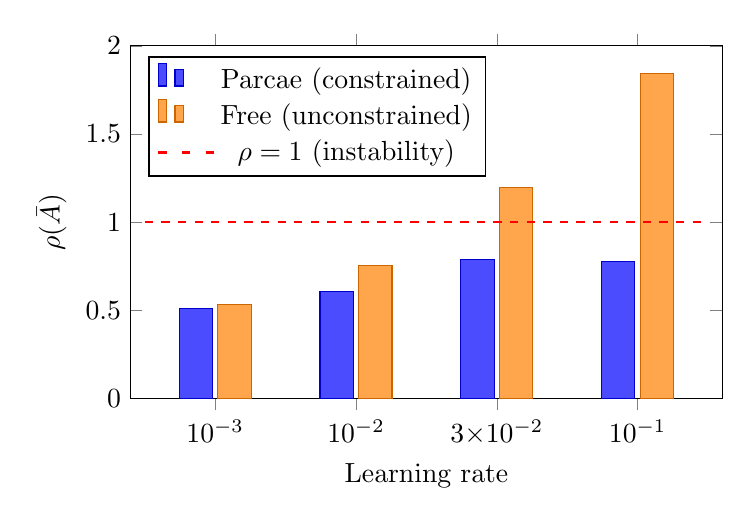
\begin{tikzpicture}
\begin{axis}[
    width=0.75\textwidth,
    height=0.5\textwidth,
    xlabel={Learning rate},
    ylabel={$\rho(\bar{A})$},
    ymin=0, ymax=2.0,
    xtick={0,1,2,3},
    xticklabels={$10^{-3}$, $10^{-2}$, $3{\times}10^{-2}$, $10^{-1}$},
    legend pos=north west,
    ybar,
    bar width=12pt,
    enlarge x limits=0.2,
]
\addplot[fill=blue!70, draw=blue!80!black] coordinates {
    (0, 0.512) (1, 0.606) (2, 0.790) (3, 0.777)
};
\addlegendentry{Parcae (constrained)}
\addplot[fill=orange!70, draw=orange!80!black] coordinates {
    (0, 0.534) (1, 0.755) (2, 1.197) (3, 1.841)
};
\addlegendentry{Free (unconstrained)}
\addplot[red, dashed, thick, sharp plot, mark=none, update limits=false, forget plot] coordinates {(-0.5, 1.0) (3.5, 1.0)};
\addlegendimage{line legend, red, dashed, thick, no markers}
\addlegendentry{$\rho = 1$ (instability)}
\end{axis}
\end{tikzpicture}
\caption{Unconstrained carry learns $\rho > 1$ at higher learning rates. The Parcae constraint (blue) is structurally bounded; the free carry (orange) crosses the instability threshold at lr $\geq 3 \times 10^{-2}$.}
\label{fig:unconstrained-carry}
\end{figure}

The constrained carry stays $\rho < 1$ at every learning rate---structurally guaranteed. The unconstrained carry is fine at low learning rate but gradient descent drives $\rho$ past 1 at higher rates (1.20 at lr=$3 \times 10^{-2}$, 1.84 at lr=$10^{-1}$), with the state norm exploding to $\sim$9,570.

Two caveats: the loss stays finite even while the state explodes, because the Coda's LayerNorm normalizes $h_T$ before the unembed---loss curves alone can hide this failure mode. And the state plateaus around $10^4$ rather than NaN-ing, because in-block LayerNorm caps per-loop growth.

\subsection{Tiny Shakespeare: Self-Correction (Weak Form)}
\label{subsec:tinyshakes}

A character-level language model ($d=32$, 4 heads, $T=4$ loops, per-channel learned $\log\_A$) was trained on Tiny Shakespeare for 150 steps. All gradients verified against central finite differences to below $10^{-6}$ (\cref{sec:reproducibility}).

\begin{table}[ht]
\centering
\begin{tabular}{@{}cccc@{}}
\toprule
Step & max($\bar{A}$) & Convergence ratio & Loss \\
\midrule
1 & 0.192 & 0.53 & 4.13 \\
50 & 0.211 & 0.20 & 3.32 \\
100 & 0.226 & 0.02 & 3.18 \\
150 & 0.233 & 0.23 & 3.05 \\
\bottomrule
\end{tabular}
\caption{Carry self-corrects on Tiny Shakespeare. The gradient $\partial L / \partial \bar{A}$ oscillates in sign, pushing mean carry back down.}
\label{tab:tinyshakes}
\end{table}

However, at max($\bar{A}$) $\approx 0.23$, the time constant is $\tau \approx 1.3$ loops---the channel converges in the first iteration. The system stayed safe because the task gave the optimizer no reason to push carry higher. The interesting equilibria remain untested.

\subsection{Full-Attention Copy Task: Falsification}
\label{subsec:full-attn}

To force the carry toward the stability boundary, we designed a synthetic task: sequences $[A][\text{pad} \times k][?]$ where the target at position ? is $A$. Solving gap $k$ should require time constant $\tau \approx k$, predicting max($\bar{A}$) $\approx 1 - 1/k$.

\begin{table}[ht]
\centering
\begin{tabular}{@{}cccc@{}}
\toprule
$k$ & Predicted max($\bar{A}$) & Learned max($\bar{A}$) & Accuracy \\
\midrule
2 & 0.500 & 0.615 & $\sim$0 \\
6 & 0.833 & 0.521 & $\sim$0 \\
8 & 0.875 & 0.659 & 0.17 \\
12 & 0.917 & 0.563 & 0.67 \\
\bottomrule
\end{tabular}
\caption{Full-attention copy: prediction falsified. $k=12$ solved best with lowest carry.}
\label{tab:full-attn-copy}
\end{table}

\textbf{The prediction is falsified.} Learned max($\bar{A}$) does not track $1-1/k$---it stays near 0.5 with no monotonic trend. $k=12$ (highest predicted, designed as ``the cliff probe'') solved best with one of the lowest carries.

The falsification reveals a fundamental architectural distinction. In a looped transformer with full self-attention and input injection, a position gap is bridged by attention in a single hop regardless of distance. The carry provides a different service---it persists the hidden state across loop iterations at a fixed sequence position (depth memory). It cannot move information across positions. The copy task recruits attention (position memory), not the carry (depth memory).

\subsection{Windowed Attention: The Carry Is Not the Memory}
\label{subsec:windowed}

To make the carry load-bearing, we restricted attention to window $w=1$ (each position attends only to itself and predecessor). Moving information across gap $k$ now requires $\lceil k/w \rceil$ loop iterations, and the carry must retain partial results between hops---a shift-register algorithm. This restores the prediction $\bar{A} \approx 1 - 1/k$ and makes $k > T \cdot w$ a genuine cliff.

Results ($T=8$ loops, $w=1$, $d=32$, curriculum stepping by 1):

\begin{table}[ht]
\centering
\begin{tabular}{@{}ccccc@{}}
\toprule
$k$ & Predicted max($\bar{A}$) & Learned max($\bar{A}$) & Accuracy & $\partial L / \partial \bar{A}$ \\
\midrule
2 & 0.500 & 0.524 & 0.91 & +0.0107 \\
3 & 0.667 & 0.533 & 1.00 & +0.0000 \\
4 & 0.750 & 0.518 & 1.00 & +0.0000 \\
5 & 0.800 & 0.505 & 1.00 & +0.0000 \\
6 & 0.833 & 0.486 & 1.00 & +0.0004 \\
\bottomrule
\end{tabular}
\caption{Windowed copy: prediction falsified decisively. Learned max($\bar{A}$) \emph{declines} from 0.524 to 0.486 as $k$ increases---opposite of the predicted climb. Gradient $\partial L / \partial \bar{A} \geq 0$ (anti-cliff) at every $k$.}
\label{tab:windowed-copy}
\end{table}

\begin{figure}[ht]
\centering
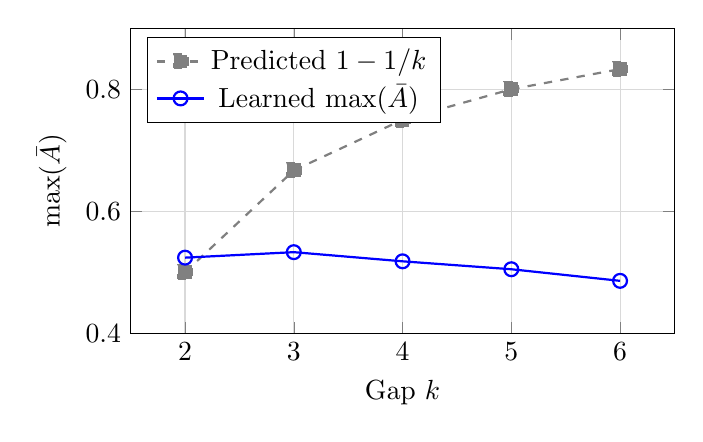
\begin{tikzpicture}
\begin{axis}[
    width=0.7\textwidth,
    height=0.45\textwidth,
    xlabel={Gap $k$},
    ylabel={$\max(\bar{A})$},
    xmin=1.5, xmax=6.5,
    ymin=0.4, ymax=0.9,
    xtick={2,3,4,5,6},
    legend pos=north west,
    grid=major,
    grid style={gray!30},
]
\addplot[gray, thick, dashed, mark=square*, mark size=2.5pt] coordinates {
    (2, 0.500) (3, 0.667) (4, 0.750) (5, 0.800) (6, 0.833)
};
\addlegendentry{Predicted $1 - 1/k$}
\addplot[blue, thick, mark=o, mark size=2.5pt] coordinates {
    (2, 0.524) (3, 0.533) (4, 0.518) (5, 0.505) (6, 0.486)
};
\addlegendentry{Learned $\max(\bar{A})$}
\end{axis}
\end{tikzpicture}
\caption{Windowed copy task: the predicted carry $1 - 1/k$ (gray) climbs toward 0.833 as gap $k$ increases; the learned carry (blue) \emph{declines} to 0.486. The block's nonlinear recurrence handles the memory; the carry is not recruited.}
\label{fig:windowed-copy}
\end{figure}

Every $k$ from 2 to 6 is solved (accuracy $\geq 0.91$, with $k=3$--6 at 1.00), demonstrating that multi-loop depth recurrence through windowed attention genuinely works. But the carry is not recruited---it \emph{declines} with increasing memory demand, the opposite of the predicted climb toward 0.833. The finer curriculum (stepping by 1 rather than by 2) was the key lever: the intermediate stages bridged the optimization landscape that a coarser $k=4 \to 6$ jump could not cross.

\subsection{Ablation: Isolating the Nonlinear Recurrence}
\label{subsec:ablation}

The windowed result shows multi-loop depth memory is used but the carry is not recruited. The two-path hypothesis attributes the memory to the block's nonlinear recurrence through $h_t$. To confirm, we ablated the block's access to $h_t$: the block receives only $e$, not the current hidden state. The carry $\bar{A} \odot h_t$ remains as the sole cross-iteration path.

Three conditions on $k=4$ copy ($T=8$, $d=24$), cold start:

\begin{table}[ht]
\centering
\begin{tabular}{@{}llccc@{}}
\toprule
Condition & Block sees $h_t$? & Attention & Accuracy & max($\bar{A}$) \\
\midrule
A: full model, windowed & yes & windowed & 1.00 & 0.517 \\
B: ablated, windowed & no & windowed & 0.09 & 0.522 \\
C: ablated, full attention & no & full & 1.00 & 0.529 \\
\bottomrule
\end{tabular}
\caption{Ablation confirms the mechanism. A vs.\ B: removing block's access to $h_t$ breaks the task. B vs.\ C: ablation removes multi-loop propagation specifically, not capacity.}
\label{tab:ablation}
\end{table}

\textbf{A vs.\ B} holds everything fixed except whether the block sees $h_t$. A solves; B fails. The cross-loop propagation runs through the block's dependence on $h_t$---the nonlinear recurrence---not the linear carry.

\textbf{B vs.\ C} holds the ablation fixed and swaps the attention mask. B fails; C solves. The ablation removed exactly one capability: multi-loop depth propagation. When full attention can bridge positions in a single hop, the ablated model is unimpaired.

This confirms the mechanism: in a looped transformer, the block's nonlinear recurrence through $h_t$---not the linear carry---provides depth memory. The carry is a convergence-rate controller, not a memory mechanism. Notably, max($\bar{A}$) does not rise in condition B to compensate for the lost nonlinear path; the carry cannot substitute.

\begin{figure}[ht]
\centering
\resizebox{\textwidth}{!}{%
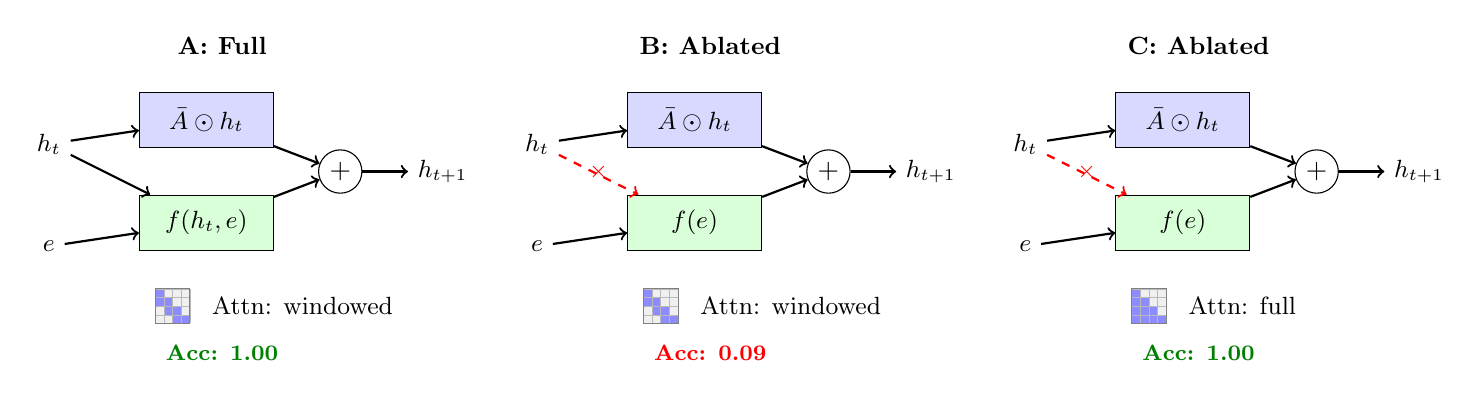
\begin{tikzpicture}[
    box/.style={draw, minimum width=1.7cm, minimum height=0.7cm, align=center, font=\small},
    arr/.style={->, thick},
    cut/.style={->, red, dashed, thick},
    sum/.style={draw, circle, minimum size=0.55cm, inner sep=0pt},
    io/.style={font=\small},
]
\newcommand{\attnicon}[3]{%
    % #1 x, #2 y (bottom-left of 4x4 grid), #3 full(1)/windowed(0)
    \begin{scope}[shift={(#1,#2)}, scale=0.11]
        \fill[gray!12] (0,0) rectangle (4,4);
        \ifnum#3=1
            \fill[blue!45] (0,3) rectangle (1,4);
            \fill[blue!45] (0,2) rectangle (2,3);
            \fill[blue!45] (0,1) rectangle (3,2);
            \fill[blue!45] (0,0) rectangle (4,1);
        \else
            \fill[blue!45] (0,3) rectangle (1,4);
            \fill[blue!45] (0,2) rectangle (2,3);
            \fill[blue!45] (1,1) rectangle (3,2);
            \fill[blue!45] (2,0) rectangle (4,1);
        \fi
        \draw[gray!55, very thin] (0,0) grid (4,4);
        \draw[gray, thin] (0,0) rectangle (4,4);
    \end{scope}
}
\newcommand{\ablunit}[7]{%
    % #1 xshift, #2 block label, #3 h_t->block live(1)/cut(0), #4 title, #5 attn full(1)/win(0), #6 acc, #7 acc color
    \begin{scope}[xshift=#1 cm]
        \node[io] (h) at (0, 0.3) {$h_t$};
        \node[io] (e) at (0, -1.0) {$e$};
        \node[box, fill=blue!15] (carry) at (2.0, 0.6) {$\bar{A} \odot h_t$};
        \node[box, fill=green!15] (block) at (2.0, -0.7) {#2};
        \node[sum] (s) at (3.7, -0.05) {$+$};
        \node[io] (out) at (5.0, -0.05) {$h_{t+1}$};
        \draw[arr] (h) -- (carry);
        \ifnum#3=1
            \draw[arr] (h) -- (block);
        \else
            \draw[cut] (h) -- (block);
            \node[red, font=\footnotesize\bfseries] at (0.78, -0.05) {$\times$};
        \fi
        \draw[arr] (e) -- (block);
        \draw[arr] (carry) -- (s);
        \draw[arr] (block) -- (s);
        \draw[arr] (s) -- (out);
        \node[font=\small\bfseries] at (2.2, 1.55) {#4};
        \attnicon{1.35}{-1.98}{#5}
        \node[io, anchor=west] at (1.95, -1.76) {Attn: \ifnum#5=1 full\else windowed\fi};
        \node[font=\footnotesize\bfseries, text=#7] at (2.2, -2.35) {Acc: #6};
    \end{scope}
}
\ablunit{0}{$f(h_t, e)$}{1}{A: Full}{0}{1.00}{green!50!black}
\ablunit{6.2}{$f(e)$}{0}{B: Ablated}{0}{0.09}{red}
\ablunit{12.4}{$f(e)$}{0}{C: Ablated}{1}{1.00}{green!50!black}
\end{tikzpicture}%
}
\caption{Ablation schematic. Each condition sums two parallel depth-memory paths---the linear carry $\bar{A} \odot h_t$ and the nonlinear block $f$---into $h_{t+1}$. In A the block reads $h_t$; in B and C that path is cut (red $\times$), so the block sees only the loop-constant input $e$. The small grid is the attention mask (banded $=$ windowed $w{=}1$, triangular $=$ full causal): B and C are the \emph{same} ablation and differ only in this mask. A (full model) solves; B fails; C (same ablation, full attention) solves. The cross-loop memory runs through the block's dependence on $h_t$, not the linear carry.}
\label{fig:ablation}
\end{figure}

\subsection{Boundary: When the Carry Is the Memory Mechanism}
\label{subsec:boundary}

The preceding experiments establish that on cross-channel tasks, gradient descent routes memory through the nonlinear block. Does a task exist where the carry's diagonal structure is efficient?

We constructed such a task: a per-channel leaky integral where the target for channel $c$ is the exponentially weighted moving average with decay $a^*_c$---exactly what a carry with $\bar{A}_c = a^*_c$ computes natively. Target decay rates spanned $a^*_c \in [0.30, 0.90]$, with $\bar{A}$ initialized at 0.5.

\begin{table}[ht]
\centering
\begin{tabular}{@{}ccc@{}}
\toprule
Target $a^*_c$ & Learned $\bar{A}_c$ & $\Delta$ from init \\
\midrule
0.30 (low) & 0.342 & $-$0.16 \\
0.50 & 0.222 & $-$0.28 \\
0.74 & 0.616 & +0.12 \\
0.90 (high) & 0.737 & +0.24 \\
\bottomrule
\end{tabular}
\caption{Diagonal-memory task: carry is recruited. Correlation $\text{corr}(\bar{A}_c, a^*_c) = 0.92$. Low-target channels dropped carry; high-target channels raised it.}
\label{tab:diagonal-memory}
\end{table}

\begin{figure}[ht]
\centering
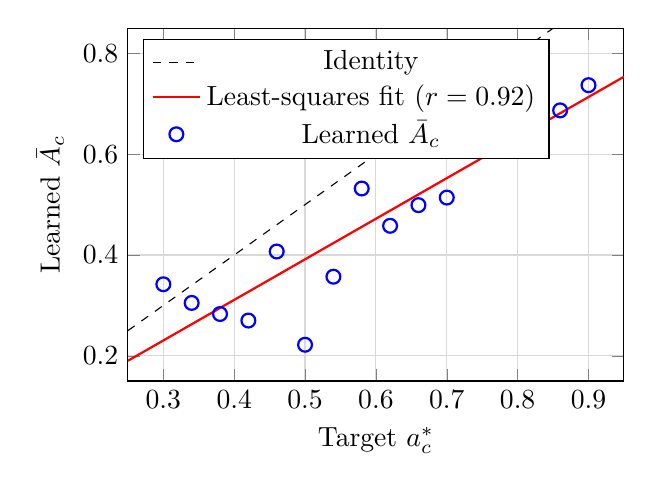
\begin{tikzpicture}
\begin{axis}[
    width=0.65\textwidth,
    height=0.5\textwidth,
    xlabel={Target $a^*_c$},
    ylabel={Learned $\bar{A}_c$},
    xmin=0.25, xmax=0.95,
    ymin=0.15, ymax=0.85,
    grid=major,
    grid style={gray!30},
    legend pos=north west,
]
\addplot[black, dashed, thin, domain=0.25:0.95] {x};
\addlegendentry{Identity}
\addplot[red, thick, domain=0.25:0.95] {0.805*x - 0.011};
\addlegendentry{Least-squares fit ($r = 0.92$)}
\addplot[only marks, mark=o, mark size=2.5pt, blue, thick] coordinates {
    (0.30, 0.342) (0.34, 0.305) (0.38, 0.283) (0.42, 0.270)
    (0.46, 0.407) (0.50, 0.222) (0.54, 0.357) (0.58, 0.532)
    (0.62, 0.458) (0.66, 0.499) (0.70, 0.514) (0.74, 0.616)
    (0.78, 0.645) (0.82, 0.679) (0.86, 0.687) (0.90, 0.737)
};
\addlegendentry{Learned $\bar{A}_c$}
\end{axis}
\end{tikzpicture}
\caption{Diagonal-memory task: learned carry $\bar{A}_c$ tracks target decay $a^*_c$ with correlation 0.92. This is the boundary case where the carry's diagonal structure matches the task structure.}
\label{fig:diagonal-memory}
\end{figure}

This is the first task where $\bar{A}$ moves substantially and tracks predicted values. Every prior task had $\text{corr} \approx 0$.

The high-target channels reached $\bar{A} = 0.74$ against target 0.90---the carry supplies per-channel structure but does not fully reach the target, with the nonlinear block supplementing the residual gain. This is a collaboration regime: the carry provides axis-aligned memory, the block handles the rest. The division of labor tracks the stability margin gradient from \cref{sec:self-stabilization}: the carry takes what it can do cheaply (low-$\bar{A}$ channels, wide margin), while the block absorbs what would be expensive for the carry (high-$\bar{A}$ channels where the margin is thin)---making the stability analysis not just a safety characterization but a prediction about how the optimizer allocates computation between the two paths.

\textbf{Caveat:} This task is artificial by design---a regression head, sequence length 1, direct input injection, with a target that is the carry's native computation. The MSE regression loss provides direct per-channel gradient signal to $\bar{A}$, an advantage not present in classification or language modeling losses. This is intentional: the experiment maps the boundary of the claim, not a natural workload.

\subsection{Synthesis}

\Cref{tab:synthesis} summarizes the experimental arc. The pattern is consistent: in cross-channel tasks, max($\bar{A}$) never moves far from its initialization regardless of memory demand ($0.19 \to 0.23$ on Tiny Shakespeare; $0.49$--$0.66$ on the copy tasks initialized at $0.5$, far below the predicted climb to $0.83$--$0.92$), while the diagonal-memory task---where the carry's structure matches the task---shows strong recruitment ($\text{corr} = 0.92$).

\begin{table}[ht]
\centering
\begin{tabular}{@{}lccc@{}}
\toprule
Task & Memory demand & max($\bar{A}$) & Carry recruited? \\
\midrule
Tiny Shakespeare & low & 0.23 & no \\
Full-attn copy ($k{=}12$) & high & 0.56 & no \\
Windowed copy ($k{=}6$) & high & 0.49 & no \\
Ablation (condition B) & --- & 0.52 & cannot compensate \\
Diagonal-memory & per-channel & 0.22--0.74 & yes ($r{=}0.92$) \\
\bottomrule
\end{tabular}
\caption{Summary of carry behavior across experiments. Cross-channel tasks do not recruit the carry regardless of memory demand; the diagonal-memory task does.}
\label{tab:synthesis}
\end{table}

The looped transformer has two depth-memory paths: the linear carry $\bar{A} \odot h_t$ (diagonal, stability-constrained) and the nonlinear recurrence through $f(h_t, e)$ (dense, universal-approximator-class). Two precisions temper this comparison. The expressivity gap is regional, not global: the increment is uniformly bounded (\cref{app:existence}), so the nonlinear path cannot represent any unbounded map---including the carry's own $h \mapsto \bar{A} \odot h$---globally; the relevant comparison is on the bounded set the dynamics actually visit, where the block's dense nonlinear class is far richer than per-channel rescaling, while the carry cannot express cross-channel interactions at any scale. And ``no stability cost'' is an empirical statement about the measured regime: the nonlinear path incurs no \emph{observed} net stability-margin cost because LayerNorm scales its Jacobian down inversely with activation norm (\cref{sec:lipschitz,sec:self-stabilization}). Given the choice, gradient descent prefers the path that is more expressive and does not deplete the directional margin.

This explains why Parcae's constraint works well: it restricts a degree of freedom the optimizer does not use for memory. The constraint remains necessary---without it, gradient descent drives $\rho > 1$ at higher learning rates (\cref{tab:unconstrained})---but it is low-cost for cross-channel workloads, which include essentially all natural-language tasks. The carry's job is stabilization, not memory.


\section{Limitations}
\label{sec:limitations}

\textbf{Scale.} All experiments use $d \le 32$ and at most 4 heads. The analytical claims are dimension-independent; quantitative behavior at larger scale is untested.

\textbf{Lipschitz estimation.} Robust estimation adds axis-aligned probes but the guarantee is empirical. Analytical bounds (possibly via structured singular value theory) would strengthen the result.

\textbf{Non-normality quantified only at toy scale.} We measure the spectral radius $\rho_{\text{spec}}(J_G(h^*))$ and the true operator norm $\|J_G\|_2$ by power iteration on Jacobian--vector products (\cref{tab:spectral,tab:seed-robustness}): $\|J_G\|_2 > 1$ in every instance that converges to a fixed point ($9/9$ seeds at $\rho = 0.3$, $8/8$ at $\rho = 0.9$; all five carries for the representative instance) while $\rho_{\text{spec}} < 1$ at every verified fixed point, so $J_G$ is non-normal and the transient step-size rebound of \cref{fig:spiral}b is confirmed rather than merely suggested; a minority of initializations never converge at all (\cref{tab:seed-robustness}). This is established at $d=32$, seq $16$, random weights; the magnitude of the non-normality gap at larger scale and after training is untested, as is the inner-gap's dependence on the attention pattern.

\textbf{Windowed copy through $k=6$ only.} Higher $k$ approaching $T=8$ remains untested, though the monotonic decline of max($\bar{A}$) suggests the pattern strengthens.

\textbf{Alternative normalizations.} The inverse-norm coupling follows from degree-0 homogeneity alone, so it holds verbatim for RMSNorm---for which the appendix bound is exact, with $P = I$ and $s = \text{RMS}$ (\cref{app:coupling})---and for ScaleNorm-style normalizers; the training-dynamics experiments, however, use LayerNorm only. Post-LN architectures would lack this implicit gain control.

\textbf{Boundary characterized, not universal.} The low-cost claim holds for cross-channel tasks. Hybrid tasks (mixing axis-aligned and cross-channel demands) remain open.


\section{Reproducibility}
\label{sec:reproducibility}

All experiments run on CPU using pure Clojure (no GPU, no native dependencies). The codebase implements dense linear algebra, multi-head causal self-attention (full and windowed), pre-LN transformer blocks, the Parcae gated recurrence (simplified and faithful modes), manual backpropagation through shared weights, and a complete training loop from scratch. All gradients verified against central finite differences across 100 test assertions (tolerance $10^{-6}$; central differences with $h = 10^{-6}$ resolve to $\sim 10^{-9}$, so the margin is real but the enforced bound is $10^{-6}$). Total compute: hours on a consumer laptop.

Code available at \url{https://github.com/clojure-finance/mythjure}, tag \texttt{paper-v1}. Namespaces: \texttt{dynamics}, \texttt{nonlinear}, \texttt{linalg}, \texttt{block}, \texttt{looped}, \texttt{lipschitz}, \texttt{analysis}, \texttt{backprop}, \texttt{data}, \texttt{copytask}, \texttt{model}, \texttt{train}.


\section{Conclusion}

We have shown that LayerNorm inside the recurrent block of a looped transformer acts as an implicit gain controller: the increment's Lipschitz constant tracks $(1-\rho)$ through the inverse-norm coupling, an affine form $\rho + \tfrac{C}{F}(1-\rho)$ with $C/F \approx 2.5$ measured near-constant across carries. This does not hold the operator-norm sum near 1---it descends from $\approx 2$ to 1 as $\rho \to 1$, and the measured operator norm exceeds 1 in every instance that reaches a fixed point---but the recurrence Jacobian is non-normal, with spectral radius below 1 at every verified fixed point. The true stability budget is the spectral margin $1 - \rho_{\text{spec}}$, widest at low carry and depleting monotonically as $\rho \to 1$; and a minority of untrained instances never converge to a fixed point at all (the fixed point exists but is not attracting), so the diagonal carry constraint is necessary but not sufficient for convergence of the full recurrence.

Training experiments reveal that in cross-channel tasks, the linear carry is not the depth-memory mechanism. The block's nonlinear recurrence is more expressive and incurs no observed stability cost, so gradient descent routes memory through it and leaves the carry at rest. This explains why Parcae's spectral-radius constraint works well in practice: it restricts a degree of freedom the optimizer does not use for memory. The constraint remains necessary---without it, gradient descent drives $\rho > 1$ at higher learning rates---but it is low-cost for the workloads looped transformers target.

We characterize the boundary of this claim: on tasks with axis-aligned per-channel structure, gradient descent does recruit the carry. Across the tasks we tested, the nonlinear block subsumes the carry whenever the task requires cross-channel or cross-position computation---an empirical dichotomy, not a proven biconditional---which covers essentially all natural-language workloads.

Verification at larger scale and on richer tasks is needed to confirm these findings generalize beyond our toy-scale experiments.


\appendix
\section{Analytical Sketch of the Inverse-Norm Coupling}
\label{app:coupling}

Consider a simplified pre-LN block whose sublayer increment is $u(h) = W_2 \cdot \text{act}(W_1 \cdot \text{LN}(h))$. In the gated recurrence (\cref{eq:recurrence}) the increment $f$ is exactly this term: the block's internal residual (identity) path is folded into the carry $\bar{A} \odot h_t$, so $f(h_t, e) = \text{Block}(h_t + e) - (h_t + e) = u(h_t + e)$ contains no identity in $h_t$. (Were $f$ to include the identity---$f = h + u(h)$---the recurrence would carry $(\bar{A} + I) \odot h_t$, with diagonal entries exceeding $1$: expansive. Its Jacobian $I + \partial u/\partial h$ has norm $\ge \|\partial u/\partial h\| - 1$ always, and $\ge 1$ whenever $\partial u/\partial h$ has an eigenvalue with nonnegative real part---generically, though not universally, non-contractive. The increment form is what keeps \cref{eq:recurrence} contractive and is what the code implements.)

The Jacobian of LN can be written exactly. For one token, with centering projection $P = I - \tfrac{1}{d}\mathbf{1}\mathbf{1}^\top$ and spread $s(x) = \sqrt{\tfrac{1}{d}\|Px\|^2 + \varepsilon}$, LayerNorm (dropping $\beta$) is $\text{LN}(x) = \gamma \odot Px/s(x)$, with
\begin{equation}
J_{\text{LN}}(x) = \frac{1}{s(x)}\,\text{diag}(\gamma)\left(P - \frac{1}{d\,s(x)^2}(Px)(Px)^\top\right),
\qquad
\|J_{\text{LN}}(x)\|_2 \le \frac{\|\gamma\|_\infty}{s(x)}.
\end{equation}
The bracketed matrix is $P$ minus a rank-one term with coefficient $\|Px\|^2/(d\,s^2) \le 1$, hence has spectral norm $\le 1$; the bound follows. So the spectral norm of the LN Jacobian is $O(1/s(h)) = O(1/\sqrt{\text{Var}(h)+\varepsilon})$: the true scale variable is the \emph{centered} per-token spread $s(h+e)$, which we abbreviate $O(1/\|h\|)$ under the RMS proxy of \cref{sec:lipschitz} ($s = \text{RMS}$ for RMSNorm, and $s \le \text{RMS}$ with equality when the per-token mean is small). The downstream linear maps $W_1, W_2$ contribute constant factors. So
\begin{equation}
\text{Lip}(f) = \|\partial u / \partial h\| = C/\|h\| + o(1/\|h\|),
\end{equation}
where $C$ collects the operator norms of $W_1, W_2$ and the activation's slope---a property of the weights, not of $\rho$.

\paragraph{The coupling is a homogeneity property.} None of this is specific to LayerNorm's algebraic form. At $\varepsilon = 0$ any such normalizer is positively homogeneous of degree $0$---$N(\alpha x) = N(x)$ for $\alpha > 0$---and differentiating this identity in $x$ gives $J_N(\alpha x) = J_N(x)/\alpha$: the Jacobian of a scale-invariant map scales inversely with the input scale, which is the entire gain-control mechanism in one line. It applies verbatim to RMSNorm ($P = I$, $s = \text{RMS}$, where the proxy of \cref{sec:lipschitz} becomes exact) and to $\ell^2$/ScaleNorm-style normalizers, with $\varepsilon$ acting only as a cutoff near the origin. Euler's homogeneous-function theorem adds a structural identity: degree-$0$ homogeneity gives $J_N(x)\,x = 0$---the Jacobian annihilates the radial direction exactly. For the $\varepsilon > 0$ LayerNorm above the identity acquires an exact correction: applying the bracketed matrix to $x$ gives $Px\,\big(1 - \|Px\|^2/(d\,s^2)\big) = Px \cdot \varepsilon/s^2$, hence
\begin{equation}
J_{\text{LN}}(x)\,x = \frac{\varepsilon}{s(x)^3}\,\gamma \odot Px,
\end{equation}
vanishing as $\varepsilon \to 0$ (verified against finite differences). This is the structural reason radial probes carry no information about the normalizer-path gain (\cref{subsec:directional}).

At the fixed point the balance identity gives the \emph{exact} scale $\|h^*\| = F/q_D(h^*)$ (\cref{eq:qd}), with $F := \|f(h^*, e)\|$, which is $O(1)$ because LayerNorm normalizes internal activations. (The worst-case form $\|h^*\| \le F/(1-\rho)$ of \cref{eq:fixed-point} recovers the $O(1/(1-\rho))$ scale bound, but---being an upper bound on the scale---it yields only a \emph{lower} bound on $\text{Lip}(f)|_{h^*}$ and is not used here; cf.\ the same point in \cref{sec:self-stabilization}.) Hence
\begin{equation}
\text{Lip}(f)\big|_{h^*} = \frac{C}{\|h^*\|} = \frac{C}{F}\,q_D(h^*)
\;\xrightarrow{\text{scalar carry}}\;
\frac{C}{F}\,(1-\rho).
\end{equation}
Thus, for scalar carry, $\rho + \text{Lip}(f) \approx \rho + \tfrac{C}{F}(1-\rho)$, an affine function of $\rho$ that reaches $1$ at $\rho = 1$ for any $C/F$ and is flat in $\rho$ precisely when $C \approx F$. The derivation fixes the affine form and the $\rho \to 1$ limit; the constant is an empirical property of the block, measured by power iteration to be $C/F \approx 2.5$ (range $2.33$--$2.78$ across $\rho \in [0.3, 0.95]$; \cref{tab:cf}), so the bound is not flat in $\rho$ and rides the boundary only as $\rho \to 1$. \qed

\paragraph{Where the approximation is loosest.} The fixed-point identity pins $\|h^*\|$, but the scale variable entering the normalizer is $s(h^* + e)$. At high carry $\|h^*\| = F/q_D \gg \|e\|$ and the distinction is immaterial; at low carry ($\rho = 0.3$, $\|h^*\| \approx 1.4F$) the injection can contribute materially to $s(h^* + e)$, biasing the effective constant downward---a plausible contributor to the true $C/F$ being lowest at low carry ($2.33$ at $\rho = 0.3$ vs.\ a peak $2.78$ at $\rho = 0.7$; \cref{tab:cf}). We measure $\|h^* + e\|/\|h^*\|$ across $\rho$ directly: it falls from $1.23$ at $\rho = 0.3$ to $1.13$, $1.05$, $1.005$, $1.002$ at $\rho = 0.5, 0.7, 0.9, 0.95$. The injection inflates the normalizer's scale variable by $\approx 23\%$ at low carry and negligibly once $\|h^*\| \gg \|e\|$---consistent in sign with the low-carry softening of the true $C/F$ (though not its full non-monotonic $\rho$-dependence, which the injection alone does not explain). The probe-implied $C/F$ of the probe record (\cref{app:probe-record}) shows a numerically similar low-carry dip, but there it is confounded by the probe's own $\approx 2.6\times$ underestimate.


\section{Existence of the Fixed Point via Boundedness}
\label{app:existence}

Existence of $h^*$ requires no contraction assumption---only the boundedness that normalization forces on the increment.

\textbf{Uniform bound on $f$.} Every path from input to output of $f$ passes through a normalizer. Per token, $\|\text{LN}(x)\| \le \|\gamma\|_\infty \|Px\|/s + \|\beta\| \le \|\gamma\|_\infty \sqrt{d} + \|\beta\|$, since $\|Px\|/s = \|Px\|/\sqrt{\|Px\|^2/d + \varepsilon} \le \sqrt{d}$---a bound independent of $x$. Downstream of the normalizers every operation preserves boundedness: attention outputs are convex combinations (softmax weights) of value vectors $W_V\,\text{LN}(x_j)$, bounded per token by $\|W_O\|_2\|W_V\|_2(\|\gamma\|_\infty\sqrt{d} + \|\beta\|)$ up to biases and head bookkeeping; the MLP increment $W_2\,\text{act}(W_1\,\text{LN}(x))$ is bounded because $|\text{act}(z)| \le |z|$ for the standard activations (ReLU, GELU, tanh). Summing the two sublayer increments and aggregating over $n$ tokens gives $\|f(h, e)\| \le B$ for a constant $B$ determined by the weights, $\gamma$, $\beta$, and the dimensions ($d$, $n$)---not by $h$.

\textbf{Invariant ball and Brouwer.} Let $r = B/(1 - \rho)$ with $\rho = \max_i \bar{A}_i < 1$. For $\|h\| \le r$,
\begin{equation}
\|G(h)\| \le \|\bar{A} \odot h\| + \|f(h,e)\| \le \rho\, r + B = r,
\end{equation}
so the continuous map $G$ sends the closed ball $B_r$ (convex, compact) into itself. Brouwer's fixed-point theorem~\citep{granas2003} yields $h^* \in B_r$ with $G(h^*) = h^*$, and in particular $\|h^*\| \le B/(1-\rho)$: the $O(1/(1-\rho))$ scale law of \cref{sec:self-stabilization} as an a priori bound rather than a consequence of the observed near-constancy of $\|f\|$ at the fixed point. A finer per-channel invariant set (a product of balls with radii $B_i/(1-\bar{A}_i)$, $B_i$ a per-channel bound on $f_i$) follows the same way, consistent with slow channels supporting larger state.

Existence is thus unconditional given $\rho < 1$. Uniqueness and local stability are separate questions, governed by the local analysis of \cref{sec:self-stabilization}: in the marginal regime this paper studies---$\rho_{\text{spec}} < 1$ at verified fixed points but no global contraction certificate---Brouwer supplies what Banach cannot. The non-convergent initializations of \cref{tab:seed-robustness} make the gap concrete: for them the fixed point guaranteed here is not attracting from the initialization used, and the iteration remains on a bounded orbit inside $B_r$ without ever settling. \qed


\section{Finite-Difference Probe Record}
\label{app:probe-record}

Before the power-iteration measurements of \cref{sec:self-stabilization}, the increment and the gated map were probed by axis-aware finite differences: random directions plus every channel axis, taking the maximum (the methodological note in \cref{subsec:directional} explains why the axis-aware upgrade over naive random probing is necessary but still insufficient). \Cref{tab:directional-margin} records those estimates, at the same block and configuration as \cref{tab:cf} ($d=32$, seq $16$, seed 7).

Read at face value, the record suggests an operator-norm contraction with a directional margin near $0.15$ that collapses as $\rho \to 1$, and an implied $C/F = (\text{bound} - \rho)/(1-\rho) \approx 1$. Both readings are probe artifacts. The top singular direction of the dense increment Jacobian $J_f$ is a coupled, non-axis-aligned direction that neither random nor channel-axis probes sample, so the probe under-estimates $\|J_f\|_2$ (hence $\|J_G\|_2$) by $\approx 2.6\times$---severely enough that the probed $\text{Lip}(G)$ falls below even $\rho_{\text{spec}}$ at every operating point. The measurements of record are the power-iteration values of \cref{tab:cf,tab:spectral}: the true $\|J_G\|_2 > 1$ at low carry, the true $C/F \approx 2.5$, and asymptotic contraction certified by $\rho_{\text{spec}} < 1$, not by any operator-norm margin. The probe's one reliable direction is the axis-aligned carry: channel-axis probes do capture it, so the per-channel worst-axis margins of \cref{sec:per-channel} stand.

\begin{table}[ht]
\centering
\begin{tabular}{@{}ccccc@{}}
\toprule
$\rho$ (carry) & Lip($G$) bound ($\rho + \text{Lip}(f)$) & Probed Lip($G$) & Directional margin & Implied $C/F$ \\
\midrule
0.3 & 0.91 & 0.85 & 0.15 & 0.87 \\
0.5 & 0.96 & 0.83 & 0.17 & 0.93 \\
0.7 & 1.00 & 0.85 & 0.15 & 1.01 \\
0.9 & 0.99 & 0.94 & 0.06 & 0.93 \\
0.95 & 1.00 & 0.97 & 0.03 & 0.93 \\
\bottomrule
\end{tabular}
\caption{\textbf{The finite-difference probe record.} Axis-aware finite-difference probe estimates of the increment and the gated map; implied $C/F = (\text{bound}-\rho)/(1-\rho)$. Retained for methodological comparison, not as a stability certificate: the probe under-estimates the true operator norms $\approx 2.6\times$ along the block's dense direction (see the discussion above and \cref{tab:cf,tab:spectral}).}
\label{tab:directional-margin}
\end{table}


\section*{Acknowledgments}

AI language model assistance was used for mathematical formalization, code generation, and manuscript drafting. The author is solely responsible for all claims, experimental design, and interpretation.

\bibliographystyle{plainnat}
\bibliography{references}

\end{document}
